\documentclass[12pt,letterpaper,oneside,openany]{book}

% --- TRU Thesis Style Guide: left margin 1.25 in, others 1 in ---
\usepackage[left=1.25in,right=1in,top=1in,bottom=1in]{geometry}
\usepackage{amsmath,amssymb,mathtools}
\usepackage{graphicx}
\graphicspath{{figures/}}
\usepackage[x11names]{xcolor}
\usepackage[colorlinks=true,linkcolor=blue!70!black,citecolor=blue!70!black,urlcolor=blue!70!black]{hyperref}
\usepackage{booktabs,tabularx,multirow,array}
\usepackage{caption,subcaption,float}
\usepackage[numbers,sort&compress]{natbib}
\usepackage{microtype,setspace}
\usepackage{algorithm,algpseudocode}
\usepackage{listings}
\usepackage[T1]{fontenc}
\usepackage{lmodern}
\usepackage{enumitem}
\usepackage{siunitx}
\usepackage{parskip}
\setlength{\emergencystretch}{3em}

\newcolumntype{L}[1]{>{\raggedright\arraybackslash}p{#1}}
\newcolumntype{C}[1]{>{\centering\arraybackslash}p{#1}}

\lstset{
  language=Python, basicstyle=\ttfamily\small,
  backgroundcolor=\color{gray!8},
  commentstyle=\color{gray}\itshape,
  keywordstyle=\color{blue!70!black}\bfseries,
  stringstyle=\color{green!50!black},
  breaklines=true, frame=single, rulecolor=\color{gray!40},
  numbers=left, numberstyle=\tiny\color{gray},
  xleftmargin=1.8em, framexleftmargin=1.8em,
  aboveskip=6pt, belowskip=6pt,
}

% TRU: body 1.5-spaced; captions and references single-spaced
\onehalfspacing
\captionsetup{font={stretch=1.0}}

% TRU: page numbers in the lower-right corner (roman in front matter, arabic in body)
\usepackage{fancyhdr}
\pagestyle{fancy}
\fancyhf{}
\fancyfoot[R]{\thepage}
\renewcommand{\headrulewidth}{0pt}
\fancypagestyle{plain}{\fancyhf{}\fancyfoot[R]{\thepage}\renewcommand{\headrulewidth}{0pt}}

\begin{document}
\frontmatter

% ===================  TITLE PAGE  ===================
\begin{titlepage}
\thispagestyle{empty}
\centering
\vspace*{0.5in}
{\large THOMPSON RIVERS UNIVERSITY\par}
\vspace{1.2in}
{\LARGE\bfseries Machine Learning-Based Scoring of Pathway-Like Gene Modules in
\textit{Arabidopsis thaliana} Using Gene Ontology Semantic Features
and SHAP Interpretability\par}
\vspace{0.8in}
{\large by\par}
\vspace{0.2in}
{\large Yuzhuo Ye\par}
\vspace{1.0in}
{\large A PROJECT SUBMITTED IN PARTIAL FULFILLMENT\\[3pt]
OF THE REQUIREMENTS FOR THE DEGREE OF\par}
\vspace{0.4in}
{\large Master of Science in Data Science\par}
\vspace{0.5in}
{\large KAMLOOPS, BRITISH COLUMBIA\par}
\vspace{0.4in}
{\large July, 2026\par}
\vspace{0.5in}
{\large Supervisor: Dr.~Yue Zhang\par}
\vfill
{\large \copyright\ Yuzhuo Ye, 2026\par}
\end{titlepage}

% ===================  ABSTRACT  ===================
\chapter*{Abstract}
\addcontentsline{toc}{chapter}{Abstract}
\noindent
\textbf{Motivation:}
Curated pathway databases (such as KEGG, AraCyc) capture only a limited fraction of \textit{Arabidopsis thaliana} genes within experimentally defined biochemical or signalling pathways, leaving many stress-responsive and co-expressed gene modules functionally unresolved. Conventional enrichment approaches, including over-representation analysis (ORA) and gene set enrichment analysis (GSEA), primarily assess enrichment against predefined gene sets and therefore offer limited support for assessing pathway-like coherence in modules absent from curated catalogues.

\noindent\textbf{Results:}
We present \textbf{PathwayML-Ath}, a supervised machine learning framework that
learns from 538 curated \textit{Arabidopsis} pathway records
(155~KEGG + 383~AraCyc), grouped into 512 unique gene-set modelling instances,
and assigns pathway-like scores to \textit{Arabidopsis} gene sets with sufficient GO annotation coverage.
Each gene set is encoded as a 69-dimensional vector comprising 60~GO term frequency
features selected from the primary training data via frequency/variance filtering and mutual-information ranking,
four pairwise GO Jaccard statistics, and five size/entropy features. In the
seed-42 reference run, XGBoost achieved nested-CV AUROC $0.838 \pm 0.023$
and held-out test AUROC/AUPRC $0.865/0.842$. A supplementary held-out comparison of
13~ML methods (Section~\ref{sec:method_comparison}; Table~\ref{tab:method_comparison}) ranked
Gradient Boosting, CatBoost, XGBoost, LightGBM and Random Forest as the five highest held-out AUROC models
(test AUROC 0.862--0.867). SHAP analysis identifies
\texttt{jaccard\_mean}, \texttt{go\_entropy} and \texttt{annotated\_gene\_count} as dominant predictors.

\noindent\textbf{Availability:}
Analysis scripts, processed data, generated tables, generated figures, and reproducibility metadata are provided in the accompanying project archive.
Raw data: KEGG (\url{https://rest.kegg.jp}), PlantCyc (\url{https://plantcyc.org}),
TAIR (\url{https://arabidopsis.org}).

\noindent\textbf{Keywords:}
\textit{Arabidopsis thaliana}; pathway-like gene-set scoring; machine learning; XGBoost;
SHAP; Gene Ontology; KEGG; AraCyc; systems biology

% ===================  CONTENTS  ===================
\tableofcontents
\listoffigures
\listoftables

\mainmatter

\chapter{Introduction}
\label{sec:intro}

Biological pathways are groups of enzymes, transporters, and regulatory factors that work together to perform specific biochemical or signalling tasks. In \textit{Arabidopsis thaliana}, curated resources such as KEGG \citep{kanehisa2023kegg} and AraCyc within the PlantCyc framework \citep{hawkins2021plant} provide 538 pathway records (155 from KEGG and 383 from AraCyc) for metabolic and signalling processes; after grouping records that share the same normalised gene membership, 512 modelling instances remain. Yet, transcriptomic and proteomic studies frequently find co-regulated gene modules that are not fully represented in these annotations \citep{obayashi2018atted,usadel2009coexpression}, so current pathway maps remain incomplete.


Common methods like over-representation analysis (ORA) and gene set enrichment analysis (GSEA) \citep{subramanian2005gsea,khatri2012ten} link gene sets to pathways by checking for enrichment in predefined lists. Their shared limitation is that undiscovered pathways absent from existing catalogues may be missed. Unsupervised methods like WGCNA \citep{langfelder2008wgcna,liesecke2018ranking} do not rely on known pathways, but they do not directly measure if genes function together. Graph neural networks learn well from network structure \citep{muzio2021biological}, but scoring pathway coherence with them needs dense protein-protein interaction maps, which remain incomplete for \textit{Arabidopsis}.


Here, we present \textbf{PathwayML-Ath}, a machine-learning framework trained entirely on \textit{Arabidopsis} pathway resources (AraCyc, KEGG, and TAIR GO annotations). Unlike methods that need protein-protein interaction graphs, our framework uses GO annotation frequencies and Jaccard overlap statistics to define functional connections. We tested 13 machine-learning algorithms, and tree-based ensemble and boosting models ranked highest for predicting pathway coherence. To make the results easier to understand, we added SHAP analysis \citep{lundberg2017unified,strudwick2025autoxai4omics}. We then evaluated PathwayML-Ath on held-out curated pathways using a systematic benchmark of constructed controls.




\chapter{Background and Motivation}
\label{sec:background_motivation}

\section{Biological pathways, gene modules, and pathway-like coherence}
\label{sec:bg_pathways_modules}

This study focuses on gene sets, but their biological meaning depends on their source. A curated pathway is a specific group of genes and proteins linked to a known process by experiments or databases. In contrast, a gene module is a broader concept based on data analysis. It can be a cluster of co-expressed genes, a group of differentially expressed genes, or any set of genes that appear related. That difference matters because a module may match a known pathway, represent only a fragment of one, combine several pathways, or point to a function that has not yet been documented at all.

PathwayML-Ath is built around that difference. Rather than trying to prove that a gene module is a new pathway, it asks a narrower question: does the gene set have a functional structure similar to known pathways? We call this property ``pathway-like coherence.'' In this study, we measure coherence by looking at Gene Ontology (GO) annotations and how similar these profiles are among the genes. If a gene set has many members sharing related GO terms, it looks more like a curated pathway than a random collection. In contrast, a mixed set of unrelated genes will show weaker coherence.

This approach is practical for plant functional genomics. Experiments often produce gene modules before pathway information is available. For example, a stress-response study might surface a cluster of genes activated by drought and heat, or a co-expression network a group of genes linked to a specific developmental stage. These modules are interesting, but they are not automatically the same as curated pathways. PathwayML-Ath helps by providing a score. High-scoring modules resemble the feature patterns of curated pathways and may be prioritised for follow-up, but their biological relevance still requires independent evidence. Low-scoring modules might be mixtures, noise, or processes that our current tools cannot capture.

\section{Curated pathway resources and the incompleteness of pathway catalogues}
\label{sec:bg_pathway_databases}

Curated pathway databases are essential for plant systems biology. KEGG provides broad pathway maps covering metabolism, genetic information processing, environmental information processing, cellular processes, and organismal systems \citep{kanehisa2023kegg}. AraCyc offers specific metabolic details for plants and is very useful for specialised metabolism in \textit{Arabidopsis} \citep{hawkins2021plant}. Comparative resources also help align pathways across different plant species. In this study, we used gene sets from KEGG and AraCyc as our positive examples. These sets represent the current standard for pathway organisation in \textit{Arabidopsis}.

However, pathway databases are necessarily incomplete. New experiments constantly update gene functions, change pathway boundaries, and find new processes. Even when a gene has GO annotations, it may not be assigned to a KEGG or AraCyc pathway. Conversely, a gene may appear in multiple pathways, especially broad ones. Therefore, these databases are best viewed as ``snapshots'' rather than complete maps. This study uses the data snapshots described in Section~\ref{sec:data}, so the results reflect this particular data build and would shift as the databases grow.

Incomplete pathway databases are the core difficulty. Standard tools can check whether a gene cluster matches a known pathway, but when there is no match they cannot tell whether the cluster's internal structure resembles a pathway. We address this with machine learning: the model is trained on known pathways as positive examples, and can then judge whether a new gene set looks like a pathway from its structure.

\section{From enrichment analysis to internal coherence scoring}
\label{sec:bg_enrichment_vs_coherence}

The most widely used pathway-interpretation methods are enrichment-based. Over-representation analysis (ORA) tests if a gene list contains more members of a known pathway than expected by chance. It typically uses statistical tests like the Fisher exact test. Gene set enrichment analysis (GSEA) tests if genes from a known pathway are clustered at the top or bottom of a ranked list \citep{subramanian2005gsea}. These methods are essential for interpreting experiments; their strengths and limitations have been reviewed \citep{khatri2012ten}, and later work has benchmarked related pathway-activity transformations \citep{zhang2020pathway}.

ORA and GSEA work well, but they answer a different question than PathwayML-Ath. They test whether a gene set matches an existing catalogue entry; PathwayML-Ath asks whether a gene set has the internal coherence of a curated pathway. The two are complementary. When both give a high score, the set is likely a known pathway or a fragment of one; a high PathwayML-Ath score without ORA support can highlight an uncurated but coherent module worth following up; and ORA significance paired with a low PathwayML-Ath score points to a set that overlaps a pathway but lacks internal coherence.

Over-claiming has to be kept in check here too. A high PathwayML-Ath score is a priority signal based on GO coherence, not proof of a newly discovered pathway; confirming a genuine pathway still needs independent experimental validation, further data, and expert judgement.

\section{Gene modules in plant transcriptomics and stress-response studies}
\label{sec:bg_plant_modules}

Plant transcriptomic studies often identify co-regulated gene modules. Co-expression databases like ATTED-II demonstrate that expression similarity helps predict gene function \citep{obayashi2018atted}. However, co-expression has limitations: it may reflect shared regulation, shared tissue specificity, broad stress response, or technical structure rather than a single pathway mechanism \citep{usadel2009coexpression}. Since plant gene annotation remains incomplete, new methods are needed to prioritise modules for experimental validation.

WGCNA is a widely used framework for identifying weighted co-expression modules \citep{langfelder2008wgcna}. It groups genes by expression similarity and labels them with colours such as blue, brown, or turquoise. These labels identify data-derived modules, not curated pathways. A WGCNA module may be enriched for a pathway, contain pathway fragments, or mix genes with shared responses but different functions. Although ranking methods and refinement of co-expression measures can improve network quality \citep{liesecke2018ranking}, a separate step is still needed for functional interpretation.
\section{Rationale for a GO-based, graph-free machine-learning approach}
\label{sec:bg_go_graphfree}

Graph-based models can in principle learn pathway structure from protein-protein interaction networks, regulatory networks, or metabolic reaction graphs, but for many plant genes these networks are incomplete and unevenly characterised. GO annotations provide a more widely available representation of gene function. The Gene Ontology was developed as a controlled vocabulary to unify biological annotation across species \citep{ashburner2000gene}, and the current GO knowledgebase continues to provide an evolving functional annotation framework \citep{geneontology2023}. TAIR provides curated \textit{Arabidopsis} annotation infrastructure that connects Arabidopsis locus identifiers with functional information \citep{berardini2015tair}.

This study uses GO annotations as a graph-free proxy for functional topology. We describe a gene set by its GO profile and by measuring the similarity between genes using Jaccard statistics. The Jaccard statistics are simple: they do not need a full interaction graph but effectively show if genes share annotation structures. This approach ensures the classifier is interpretable, reproducible, and suitable for SHAP-based analysis.

\section{Negative examples and benchmark design}
\label{sec:bg_negatives}

A supervised classifier requires negative examples, but negative examples are difficult to define biologically. A gene set that is absent from KEGG or AraCyc does not mean it is not a pathway; it may be an incomplete pathway, an uncurated module, or a condition-specific response programme. This mirrors the challenge in protein function prediction where the absence of an annotation may reflect incomplete knowledge rather than biological absence \citep{radivojac2013community}. For this reason, the negative class in PathwayML-Ath represents synthetic contrast examples rather than experimentally verified non-pathways.

The benchmark used in this thesis follows the four-class constructed-negative design implemented in the project code: random gene sets, shuffled pathways, partial pathways, and cross-pathway mixtures. Each tests a specific failure mode. Random gene sets provide an easy background null. Shuffled pathways destroy membership while preserving size. Partial pathways test whether the classifier distinguishes complete curated pathways from incomplete pathway fragments. Cross-pathway mixtures check if mixed signals produce false positives. 
These negatives vary in difficulty, so they need cautious interpretation: partial pathways in particular may retain real biological coherence, and a high score on a partial fragment is not necessarily an error. This benchmark is therefore best understood as a stress test of a pathway-like scoring model rather than as a catalogue of confirmed non-pathways.

Because negatives are difficult to define, evaluation uses several diagnostics. Training-only nested cross-validation measures the effect of class balance, while ablation tests dependence on GO frequency, Jaccard, and size/entropy features. Performance is also reported separately for each negative type.

\chapter{Literature Review}
\label{sec:literature_review}

\section{Gene Ontology and functional representation}
\label{sec:lit_go}

GO-based representations are widely used in computational biology because GO provides a structured vocabulary for biological processes, molecular functions, and cellular components \citep{ashburner2000gene,geneontology2023}. In pathway analysis, they are valuable because they assign functional profiles to genes missing from curated databases. GO annotations are imperfect: incomplete, and sometimes biased towards well-studied genes. Nevertheless, they provide a practical starting point for building interpretable feature representations in organisms such as \textit{Arabidopsis}.

Several GO-based similarity measures exist. Some methods evaluate ontology terms by how specific (information-rich) they are, while others use the direct overlap of GO term sets. PathwayML-Ath uses the overlap method (Jaccard statistics) because it is transparent, simple, and easy to interpret: two genes are similar when they share a larger fraction of their GO annotations. The model also includes GO frequency features, which describe the overall composition of the gene set rather than the links between individual genes.

Feature selection is needed because raw GO spaces are high-dimensional and contain many very rare or broad terms. The present pipeline removes terms that annotate too few genes or too many genes, removes low-variance terms, and then ranks the rest using mutual information with the class label. Mutual-information feature selection is a standard way to select informative features in high-dimensional biological data \citep{dingpeng2003}, and sparse or parsimony-oriented feature selection methods are often used to reduce noise in biological classifiers \citep{tibshirani1996regression}. In PathwayML-Ath, the top 60 selected GO terms are not manually chosen; they are selected by this filtering and ranking procedure.

\section{Pathway enrichment, pathway activity, and gene-set interpretation}
\label{sec:lit_enrichment}

ORA and GSEA are essential for interpreting gene expression and gene-list experiments. ORA provides a straightforward test of whether a submitted gene list is enriched for an existing pathway. GSEA applies this concept to ranked genome-wide lists and has become a standard approach for analysing expression signatures \citep{subramanian2005gsea}. Reviews and protocols emphasise that pathway analysis is not a single method but a family of approaches with different assumptions about input type, pathway catalogue, and statistical null model \citep{khatri2012ten}. More recent work has benchmarked pathway activity transformations and gene-set scoring in high-dimensional expression data \citep{zhang2020pathway}.

These methods are complementary to PathwayML-Ath. Enrichment methods test if a gene list is statistically related to known pathways. PathwayML-Ath evaluates whether the submitted gene set has internal GO-based coherence similar to curated pathways. It is most useful for unranked gene sets, where no genome-wide ranked list is available, and for exploratory module analysis in which the gene set may not match a single curated pathway.

\section{Co-expression modules and network-based function inference}
\label{sec:lit_networks}

Network-based approaches provide another route to function inference. WGCNA identifies modules of co-expressed genes using weighted correlation networks \citep{langfelder2008wgcna}. Plant-specific studies show that co-expression can assist gene-function discovery, especially when curated functional annotations remain incomplete \citep{obayashi2018atted,usadel2009coexpression,liesecke2018ranking}. Network-integration methods combine multiple association networks to support gene-function prediction, and community-wide evaluations like CAFA have shown that computational prediction is promising but also difficult \citep{radivojac2013community}.

Deep learning has advanced network-based function inference, and graph neural networks are increasingly used for biological network analysis \citep{muzio2021biological}. However, these methods often require dense networks and carefully curated graph structure. PathwayML-Ath deliberately takes a simpler graph-free route so that pathway-like coherence can be evaluated from GO annotation alone.

\section{Machine learning for tabular biological data}
\label{sec:lit_ml_tabular}

The feature representation in PathwayML-Ath is a structured tabular vector. For such data, tree-based models and gradient boosting serve as strong baselines. Random forests aggregate many decision trees, each grown on a bootstrap sample and a random subset of features; decorrelating the trees this way lowers the variance of their averaged prediction \citep{breiman2001random}. By contrast, gradient boosting builds the ensemble one tree at a time, with each new tree correcting the errors of the current model, which lets it capture complex feature interactions but requires careful tuning to prevent overfitting \citep{friedman2001greedy}. XGBoost is an efficient version of gradient boosting that penalises complex trees and uses second-order gradient information to choose better splits, which has made it a standard choice for tabular prediction \citep{chen2016xgboost}. LightGBM and CatBoost provide alternative boosting implementations that can be highly competitive under different feature and sample-size conditions \citep{ke2017lightgbm,prokhorenkova2018catboost}. Empirical studies indicate that tree-based models often remain strong on tabular datasets compared with deep neural networks \citep{grinsztajn2022why}.

The supplementary 13-model comparison is therefore best read as model-selection context; it is not the central scientific contribution. It checks whether the final feature representation supports competitive classification across model families and whether XGBoost is a reasonable reference model. The main contribution is the pathway-coherence formulation, the GO/Jaccard feature engineering, and the validation design---not a claim that XGBoost is a universally optimal classifier.

Class balance is also relevant. The primary benchmark uses a 1:1 positive-to-negative ratio, and the ratio comparison evaluates how AUROC and precision--recall performance change as the negative class grows. Literature shows that class proportions can influence threshold-dependent metrics and precision-recall behaviour \citep{japkowicz2002class}. AUROC is often stable under imbalance, while AUPRC can be more informative when the positive class is the class of interest \citep{saito2015precision}. For this reason, the thesis reports AUROC, raw AUPRC, and AUPRC rescaled relative to its prevalence-dependent random baseline.

\section{Explainability and biological interpretation}
\label{sec:lit_xai}

A pathway-like score is useful only if it can be interpreted. SHAP provides a unified framework for assigning feature-level contributions to model predictions \citep{lundberg2017unified}. In biology, explainability matters because a model score should guide hypothesis generation rather than replace biological reasoning. Interpretability lets users judge whether a prediction is biologically plausible before acting on it. Automated XAI workflows for omics and tabular data further demonstrate the growing importance of interpretation in biological machine learning \citep{strudwick2025autoxai4omics}.

In PathwayML-Ath, SHAP is used to identify whether predictions are driven by pairwise GO coherence, broad size or entropy features, or specific GO term frequencies. The score is interpretable precisely because of this: a candidate that scores highly on a biologically coherent GO profile is more compelling than one carried mainly by gene-set size. Similarly, a low-scoring gene set with a significant ORA result may reflect overlap with a known pathway but weak internal coherence across the full module.

\section{Foundation models, multi-omics representations, and future directions}
\label{sec:lit_future}

GO-based features are interpretable and reproducible, but they do not capture all biological information. Protein language models such as ESM-2 provide sequence-derived representations that may help characterise poorly annotated proteins \citep{lin2023evolutionary}. Transcriptomic and single-cell foundation models are beginning to learn richer representations from large-scale expression data, and future multimodal models may bring together sequence, expression, structure, perturbation, and imaging data. Deep-learning methods for plant genome sequences could also help represent genes that current GO annotation covers poorly.

Multi-omics integration is another likely direction. Integrating transcriptomic, proteomic, metabolomic, and network layers can improve functional module discovery and disease or phenotype stratification in other biological systems \citep{hasin2017multiomics}. However, using richer data also requires more careful validation. Therefore, this thesis focuses on a GO-based method first. This approach is transparent, reproducible, and easy to interpret, providing a solid baseline before moving on to more complex multimodal models.

\section{Evaluation metrics, class imbalance, and benchmark interpretation}
\label{sec:lit_metrics}

The choice of evaluation metric strongly affects how we interpret a classifier. AUROC measures the probability that a randomly chosen positive sample receives a higher score than a randomly chosen negative sample. It is useful for comparing ranking ability across thresholds, but it can appear stable even when the positive class becomes rarer. Precision-recall analysis is often more informative when we focus on the positive class, because it shows how many high-scoring candidates are true positives \citep{saito2015precision}. This is why PathwayML-Ath reports both AUROC and AUPRC. A model with acceptable AUROC but modest AUPRC may still be useful for prioritisation, but it should not be treated as a high-confidence discovery engine.

Class balance is a second issue. The 1:1 through 1:5 ratios were compared by nested CV within the outer training set. The 1:1 ratio had the highest normalised AUPRC and F1, while its AUROC stayed close to the more negative-heavy settings. Read alongside baseline-adjusted AUPRC, the 1:1 setting comes out ahead, even though the settings look similar on AUROC alone \citep{saito2015precision}; the outer test set was only touched after this choice was fixed.

\section{Reproducibility, data provenance, and version control}
\label{sec:lit_reproducibility}

Reproducibility is a central issue in pathway-level machine learning because the results depend on multiple moving parts. These include pathway database snapshots, GO annotation versions, gene identifier parsing, negative-sampling rules, feature-selection procedures, random seeds, and model hyperparameters. Small changes in any of these steps can alter the selected GO features or the resulting scores. This thesis therefore treats the generated tables and manifest files as part of the scientific record, rather than mere computational by-products.

All results reported here are computed directly from source-file parsing of the KEGG, AraCyc, and TAIR GO files. Every reported number---dataset counts, performance metrics, and diagnostic results---is taken from the generated tables rather than transcribed by hand. Each value can therefore be traced back to a specific generated table. The LaTeX source, generated outputs, software versions, and code archive are kept together, so that any numerical claim in the text can be checked against the files that produced it.

\section{Positioning of PathwayML-Ath}
\label{sec:lit_positioning}

The literature suggests a clear niche for PathwayML-Ath. Enrichment methods test relationships to existing pathway catalogues. Co-expression methods identify modules but do not directly score pathway-like functional coherence. Graph and foundation models can provide rich representations but require more data and may be less interpretable. PathwayML-Ath fills this gap: it uses public GO annotations to create transparent features, trains a supervised classifier on curated \textit{Arabidopsis} pathways, and produces a pathway-like coherence score for \textit{Arabidopsis} gene sets with sufficient GO annotation coverage.

That positioning shapes how the results should be read. A high score indicates resemblance to curated pathways under the GO/Jaccard feature representation; it is not a discovery of a new pathway by itself. A low score does not prove biological irrelevance, because GO annotations may be incomplete and some true biological processes may not be captured by current features. PathwayML-Ath is therefore best used as one component of a workflow that includes enrichment analysis, GO/SHAP interpretation, literature review, network evidence, and experimental validation.




\section{Pathway interpretation as a modelling problem}
\label{sec:bg_why_thesis}

Pathway interpretation is usually treated as a final annotation step, but it is better seen as a modelling task in its own right. In a typical workflow, a researcher obtains a gene list from differential expression, clustering, co-expression, or genome-wide association analysis, submits it to an enrichment tool, and interprets the most significant terms. This method leaves several questions unanswered. It does not reveal if the gene list is coherent, or if it represents a single functional programme or a mixture of unrelated programmes, or if a lack of a significant enrichment result reflects biological novelty, incomplete annotations, or just poor overlap. These questions are important for plant stress biology. In plants, stress responses often combine hormone signalling, detoxification, transport, metabolism, and regulation into modules that do not fit exactly into one curated pathway entry.

The thesis treats pathway interpretation as a supervised representation-learning problem on gene sets. Here the curated pathways are not just labels; they are examples of what a pathway-like gene set looks like in a GO-derived feature space. This reframing changes the question being asked. An enrichment method checks how a query set lines up against one database entry; PathwayML-Ath instead compares the internal structure of that set against the structure it has learned from many pathways at once. In practice the two are used together.

That is why the study pays close attention to negative construction and to feature attribution. If the negatives are too easy, a classifier may learn trivial shortcuts. If the features are uninterpretable, a high score will be difficult to use biologically. If results are interpreted too strongly, model scores might be mistaken for discovery claims. The thesis deliberately positions PathwayML-Ath between these extremes. It is intended to help prioritise and interpret gene modules, not to replace biological curation or experimental validation.

\section{Practical problem: interpreting gene lists that are not pathway entries}
\label{sec:bg_practical_problem}

A common challenge in plant genomics is that the primary output of an experiment is often a gene list rather than a pathway. An RNA-seq experiment yields sets of upregulated and downregulated genes; clustering a time-course produces groups with similar temporal patterns; and in a co-expression network, WGCNA or related methods return colour-labelled modules with shared expression \citep{langfelder2008wgcna,obayashi2018atted,liesecke2018ranking}. In each case, the gene list is useful, but its biological interpretation is not automatic.

The term ``module'' is used deliberately broadly here. It may refer to a co-expression module, a differential-expression cluster, a network community, or a manually assembled set. In contrast, a biological pathway implies a specific mechanism where members work together in a defined biochemical or signalling process. The aim of PathwayML-Ath is to estimate whether a module has features resembling curated pathways. It does not claim that all high-scoring modules are pathways, nor that all low-scoring modules are biologically unimportant. Instead, it provides a structured, reproducible, GO-based score. The score can be combined with enrichment analysis, literature review, and experimental knowledge.
\section{Why GO annotations are suitable but imperfect}
\label{sec:bg_go_suitable_imperfect}

Gene Ontology (GO) provides a controlled vocabulary for molecular function, biological process, and cellular component \citep{ashburner2000gene,geneontology2023}. This is attractive for cross-pathway representation because the same GO term can connect genes that occur in different pathway catalogues or experimental contexts. GO annotations also allow the model to work without expression values, protein sequences, or network edges for the submitted gene set. In this project, GO is used in two ways. First, the frequency of GO terms represents the functional composition of a gene set. Second, pairwise Jaccard statistics summarise how much functional annotation is shared among genes.

However, GO annotations have limitations. Annotation depth varies across genes: some carry many experimentally supported annotations, others only sparse or electronically inferred ones. GO terms also vary in specificity, with very general terms such as ``biological process'' or ``cellular process'' too broad to identify pathways and extremely rare terms unstable as predictors. The filtering procedure used in this thesis addresses this by removing terms that are too rare or too broad before selection. Nevertheless, model predictions are still limited by the quality and completeness of the GO data.

The use of GO is a practical modelling decision, not a claim that it captures all pathway biology. Important pathway relationships are found in metabolite flow, protein interactions, location, or regulation. These are not fully represented by GO frequency and Jaccard features. A future extension could combine GO features with co-expression networks, protein models, reaction graphs, or metabolomic data. The current thesis deliberately begins with GO because it is interpretable, widely available, and sufficiently structured to support a reproducible first-generation classifier.

\section{Why negative examples require explicit design}
\label{sec:bg_negative_design}

In biological prediction, true negative examples are difficult to define. The absence of a pathway annotation does not necessarily mean that a set of genes is biologically unrelated; it may simply mean that the process has not been curated. This is similar to the open-world problem in protein function prediction, where missing annotations are not evidence of absence \citep{radivojac2013community}. For this reason, this work treats negatives as synthetic controls, not as experimentally verified non-pathways.

This analysis uses four negative classes: random gene sets, shuffled pathways, partial pathways, and cross-pathway mixtures. Each class probes a different aspect of the classification task. Random sets give an easy background comparison; shuffled pathways preserve size while disrupting membership; partial pathways test the effect of incompleteness; and cross-pathway mixtures test whether signal from different pathways can be mistaken for a single coherent one. Although this scheme is not perfect, it is more informative than using only purely random negatives.

Negative construction also affects how performance should be interpreted. A high AUROC against a mixed negative benchmark does not mean that the classifier can reject every difficult borderline set. Performance against cross-pathway mixtures or partial pathways may be lower than performance against random controls. Therefore, this thesis reports model performance as a benchmark under a defined design rather than as an absolute measure of biological pathway detection. This interpretation is especially important because real experimental modules may resemble the harder negative types more than they resemble random gene sets.

\section{Research questions}
\label{sec:bg_research_questions}

The thesis is organised around four research questions. First, can GO frequency and pairwise GO Jaccard statistics distinguish curated \textit{Arabidopsis} pathways from constructed non-pathway-like gene sets? Second, do gradient-boosted tree models offer a practical advantage over linear and non-linear baseline classifiers for this tabular representation? Third, which feature groups contribute most to pathway-like scoring? Fourth, how stable are results across class-balance settings and repeated nested cross-validation?

These questions span prediction, interpretation, and methodology. A high score is only useful once its biological meaning is clear, and interpretation only matters if the model can actually separate held-out pathways from controls, so the work ties the two together through a reproducible pipeline, interpretable features, a systematic model comparison, and a cautious way of reading gene-set scores.

\section{Thesis contributions}
\label{sec:bg_contributions}

This thesis makes four contributions. First, it introduces a GO-based feature representation for pathway-like gene-set scoring in \textit{Arabidopsis}. The representation combines GO term frequencies with pairwise GO Jaccard statistics and size/entropy features. Second, it evaluates multiple machine-learning models under the same feature representation, showing that tree-based ensemble and boosting models are competitive for this tabular biological task. Third, it provides a structured validation framework including held-out testing, nested class-ratio comparison, ablation, negative-type analysis, and SHAP interpretation. Finally, it delivers a reproducible project structure linking generated code outputs to the LaTeX manuscript.

The value of these contributions lies in the workflow they produce, not in a single headline AUROC. A researcher can use PathwayML-Ath to check whether an unranked gene list resembles curated pathways in its GO features, and read the output as a prioritisation signal rather than a finished biological claim. That makes the framework well suited to exploratory plant functional genomics, where many experimental modules need interpretation but only a few can be carried forward to experimental validation.

\section{Structure of the thesis}
\label{sec:bg_structure}

The remainder of this thesis is structured as follows. The Literature Review situates the project within GO-based functional representation, enrichment analysis, co-expression networks, machine-learning models for tabular biological data, and explainable AI. The Methods section describes the data sources, feature construction, negative-sampling scheme, model training, model comparison, and SHAP analysis. The Results section reports the dataset summary, model comparison, ratio sensitivity, feature-selection stability, SHAP features, and ablation. The Discussion interprets the results, explains the role of PathwayML-Ath alongside ORA and GSEA, and outlines limitations and future work. The appendices provide reproducibility, terminology, and interpretation notes that support the main text.

\section{GO-based functional representation beyond enrichment}
\label{sec:lit_go_extended}

GO-based analysis has traditionally been associated with enrichment testing, but GO annotations can offer more than just binary labels. Each gene is a set of GO annotations, and a gene set is defined by their distribution. This view is central to PathwayML-Ath. Rather than using GO only to label enriched categories, the model uses GO as an input feature space. GO term frequency features encode which biological functions are common in the gene set, while Jaccard statistics encode how similar the member genes are to one another.

This use of GO has several advantages. It is specific enough to capture plant biology using TAIR annotations \citep{berardini2015tair}, but general enough to permit comparison across pathways and modules. It is interpretable because each selected feature maps to a GO term. It also enables graph-free similarity, meaning genes need not be linked by protein interactions to be similar. These advantages show why GO remains practical, even with modern protein models and graph neural networks.

The limitations are equally important. GO annotations are curated and therefore incomplete; they also reflect the organism's research history. Well-studied genes and processes have richer annotation, while poorly characterised genes may be underrepresented. GO also does not directly encode reaction order, metabolite flow, regulatory causality, or temporal dynamics. GO-based coherence is thus a proxy for pathway structure, not a full mechanistic model. This thesis treats that proxy as useful because it is transparent and reproducible, but it should be combined with other evidence.

\section{Enrichment analysis and pathway activity methods}
\label{sec:lit_enrichment_extended}

ORA and GSEA are the main methods for connecting gene lists and expression signatures to known biological processes \citep{subramanian2005gsea,khatri2012ten}. They succeed because they ask a simple question: is a known gene set over-represented in the list, or enriched at one end? These methods are appropriate when the goal is to check for membership or enrichment. However, they are less appropriate when the question is about internal coherence of a gene set that may not match a single known pathway.

Pathway activity methods extend enrichment ideas by turning expression matrices into pathway features. Studies show that pathway activity methods can help interpret complex data and reduce noise \citep{zhang2020pathway}. However, these methods usually assume that pathway definitions are already available. PathwayML-Ath is complementary: it uses curated pathways as training examples but scores the structure of a new gene set, rather than measuring the activity of a predefined pathway.

These approaches differ mainly in their inputs and outputs. ORA starts from an unranked gene list and flags enriched terms, GSEA does so for a ranked genome-wide list, and pathway-activity methods turn an expression matrix into scores for pathways that are already defined. PathwayML-Ath also takes an unranked gene list, but returns a single pathway-like coherence score. It therefore sits beside enrichment analysis instead of replacing it, answering a related but separate question.

\section{Co-expression networks and functional module discovery}
\label{sec:lit_coexpression_extended}

Co-expression analysis is one of the main sources of gene modules in plant biology. WGCNA identifies genes with correlated expression profiles and is a standard tool for RNA-seq and microarray studies \citep{langfelder2008wgcna}. Plant resources like ATTED-II show that co-expression can predict gene function and generate hypotheses \citep{obayashi2018atted}. Reviews highlight both the power and limitations of these tools: co-expression suggests coordinated regulation, but it does not confirm pathway membership or mechanistic interaction \citep{usadel2009coexpression}.

This is exactly why PathwayML-Ath is useful for scoring modules. A co-expression module may represent a known pathway, a pathway fragment, a mixture of biological processes, or just a regulatory pattern. GO-based scoring adds a different layer of evidence: it checks if the genes share functional annotations like curated pathways do. In practice, a researcher can first find modules with WGCNA. Then, they can use ORA, PathwayML-Ath, and SHAP to decide if a module is a known pathway, a pathway-like cluster, or a mixed response.

\section{Network-based function prediction and graph learning}
\label{sec:lit_networks_extended}

Network-based methods have long been used to predict gene and protein function by integrating different sources of evidence. Recently, graph neural networks (GNNs) have improved these predictions and biological network analysis by learning from structured interaction graphs \citep{muzio2021biological}. These methods are attractive for pathway-coherence scoring because pathways are not just lists of genes. Instead, they are structured systems with reactions, regulations, and interactions.

However, graph methods require a suitable graph. For many plant genes, especially in stress-response contexts, experimental interaction data is incomplete. If a GNN is trained on an incomplete network, the result may reflect data availability as much as biology. PathwayML-Ath avoids this by using GO annotations and pairwise similarity. The graph-free design is a practical choice for cases where complete networks are unavailable, not a claim that it beats graph learning where good networks exist.

The framework could later be extended to include network features. For example, pairwise GO Jaccard statistics could be complemented with co-expression density, protein interaction density, or graph embedding features. A rigorous comparison would require the same train/test splits and the same negative controls. Until such data are available, the GO-based model offers a transparent baseline for pathway coherence.

\section{Machine learning on tabular biological features}
\label{sec:lit_tabular_extended}

The feature matrix in this thesis is tabular. Each gene set is described by numeric descriptors such as GO term frequencies, Jaccard summaries, entropy, and size. For tabular data, tree ensembles and gradient-boosted decision trees often perform well because they capture non-linear feature interactions without requiring large sample sizes \citep{breiman2001random,friedman2001greedy,chen2016xgboost,ke2017lightgbm,prokhorenkova2018catboost,grinsztajn2022why}. This is why the thesis compares classical, ensemble, boosting, and neural-network models rather than choosing a single classifier.

The comparison is a supporting analysis, not the headline result. The goal is not to crown the single best algorithm, only to show that the chosen model works well with the current features and data. In these tests the top five models by AUROC---Gradient Boosting, CatBoost, XGBoost, LightGBM, and Random Forest---are all tree-based. That supports using a tree model downstream and indicates the result does not hinge on one algorithm.

\section{Explainability as a requirement for biological use}
\label{sec:lit_xai_extended}

Biological prediction models are useful only when their predictions can be interpreted in relation to biological mechanisms. A model that assigns a high score to a gene module without indicating why it did so is difficult to use for hypothesis generation. SHAP provides a feature-attribution framework that breaks down the prediction into contributions from each input feature \citep{lundberg2017unified}. In biological machine learning, explainability matters because researchers must connect model behaviour to domain knowledge \citep{strudwick2025autoxai4omics}.

In PathwayML-Ath, SHAP values support two levels of interpretation. Globally, they identify which features drive the classifier across the held-out test set. Locally, they can help interpret a particular candidate gene set by indicating whether its score is driven by internal Jaccard coherence, functional entropy, gene-set size, or specific GO term frequencies. This does not make the model fully mechanistic, but it helps identify whether predictions are biologically plausible. For example, if a photosynthesis gene set gets a high score because of relevant GO features, the score is easier to interpret than if it were driven only by size.

\section{Synthesis of the literature and the project gap}
\label{sec:lit_synthesis}

The reviewed literature suggests a clear gap. Enrichment analysis interprets overlap with known gene sets well; co-expression analysis is effective at identifying modules from expression data; network and graph-learning methods work when dense interaction graphs are available; and foundation models offer promising representations for genes and proteins. However, there is still a need for an interpretable, GO-based method. Such a method should score an unranked gene list for pathway-like coherence without requiring a ranked expression profile or a complete interaction graph.

PathwayML-Ath addresses this gap by combining curated pathway examples, GO annotation features, pairwise Jaccard statistics, tree-based classification, and SHAP interpretation. Its scope is intentionally narrow. Instead of discovering pathways, it prioritises gene sets for closer analysis, and is designed to work alongside ORA and GSEA, not to displace them. It also does not fix the gaps in current annotation; what it offers is a way to put that annotation to work within a reproducible scoring framework. Those limits are where the contribution of this thesis lies.


\chapter{Methods}
\label{sec:methods}

\section{Data sources and preprocessing}
\label{sec:data}

KEGG \textit{Arabidopsis thaliana} (ath) pathway names and pathway--gene
associations were downloaded through the KEGG REST API on 25 May 2026, when
Release 118.1 was current. After duplicate assignments were collapsed, 155
KEGG pathways met the five-gene minimum.

The AraCyc source was AraCyc 18.0.0 from PMN Release 16, released on
30 July 2024. The analysis used the PlantCyc flat file
\texttt{aracyc\_pathways.20251021}. The date in this file name is
21 October 2025; it is the flat-file date, not the AraCyc version. The file was
downloaded and archived on 25 May 2026. Filtering retained 383 pathways with at
least five unique AGI locus IDs (format AT\textit{n}G\textit{nnnnn}). Combined,
the source collection comprised 538 pathway records. Records with identical
normalised gene membership were grouped into one modelling instance while all
identifiers were retained as aliases. This produced 512 unique gene-set
instances: 155 in the KEGG stratum and 357 in the AraCyc stratum. There were
20 exact-duplicate groups containing 26 extra records. Identical gene lists can
arise when current superpathway and subpathway annotations coincide, when
separate reversible-reaction records use the same genes, or when annotation is
incomplete. The modelling instances ranged from 5 to 2,429 genes (median 15,
mean $39.2 \pm 132.2$ genes; Figure~\ref{fig:datastats}).


\begin{figure}[H]
\centering
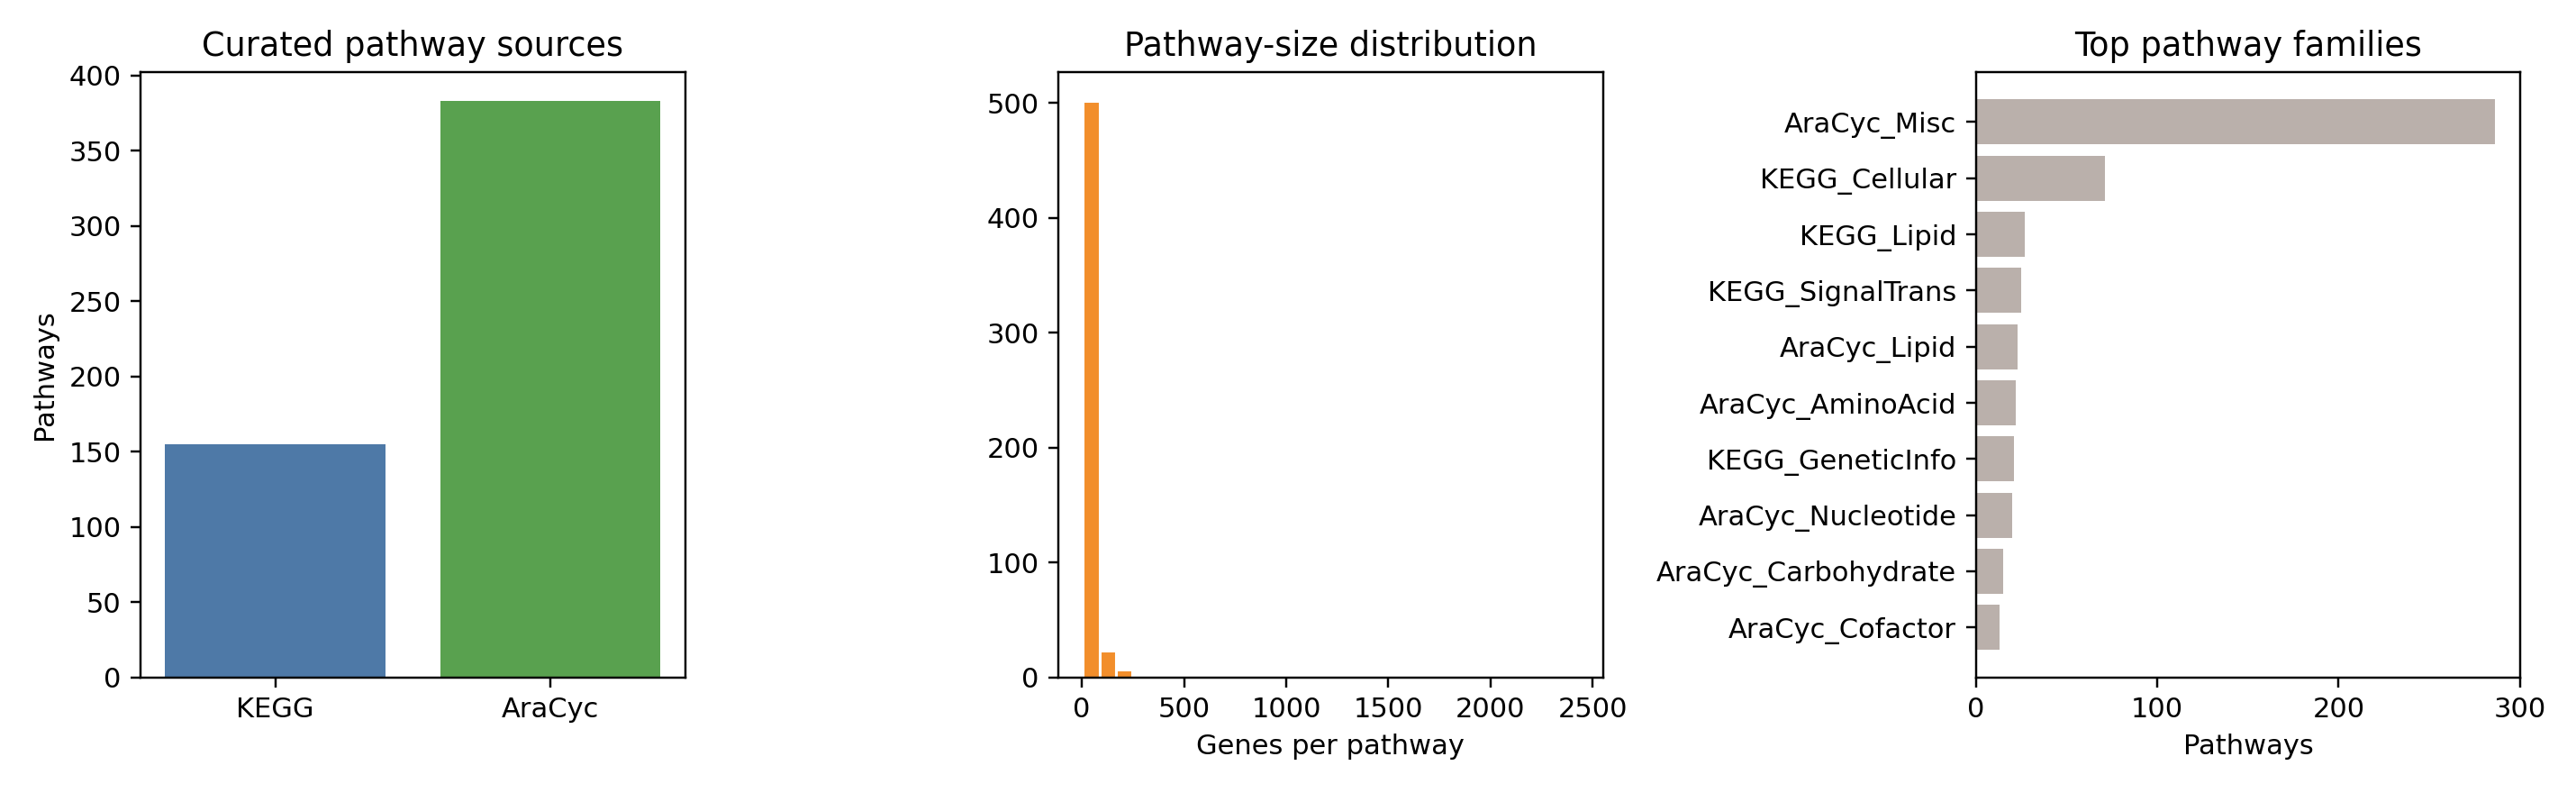
\includegraphics[width=\textwidth]{Fig5_datastats.png}
\caption{\textbf{Dataset statistics.}
The dataset figure summarises the 512 unique gene-set modelling instances:
155 in the KEGG stratum and 357 in the AraCyc stratum, their right-skewed size
distribution, and the exact grouping of 538 source records into 512 instances.
GO feature-selection counts are reported in the text and Table~\ref{tab:s5_data}.}
\label{fig:datastats}
\end{figure}

The GO annotations came from the TAIR public data release
\texttt{TAIR\_Data\_20250331}; its \texttt{ATH\_GO\_GOSLIM.txt} file reports a
last-update date of 1 April 2025 and was downloaded and archived with the
project data on 25 May 2026. Collapsing duplicate gene--GO pairs produced
28,998 GO-annotated genes and 7,067 unique GO terms. Pathway-gene
coverage in the current data build was 97.97\% (7{,}184 of the 7{,}333 genes appearing in the 538 source records carry at least one GO annotation).

A three-stage filtering and feature-selection procedure was applied to remove noisy or overly general GO terms while retaining informative features. First, a label-free frequency filter excluded terms annotating fewer than 20 genes or more than 30\% of the 28,998 annotated genes (7,067~$\rightarrow$~829). The positive instances were then divided into primary training and outer-test sets, and controls were generated independently on each side. Second, a variance filter fitted only to the 818 primary training records removed terms below the 15th percentile of variance (829~$\rightarrow$~704). Finally, scikit-learn's mutual-information estimator \citep{pedregosa2011scikit} ranked the remaining terms against the primary training labels, and the top 60 were kept (704~$\rightarrow$~60). This ranks terms on relevance alone; unlike mRMR~\citep{dingpeng2003}, it does not penalise redundancy between selected terms. The 206 outer-test records were not used for variance filtering or mutual-information ranking. These 60 terms were used for the final held-out model, model comparison, SHAP analysis, and ablation. For repeated cross-validation, the variance and mutual-information steps were rerun within each fold using only that fold's training records.



\begin{table}[H]
\centering
\caption{\textbf{Data sources, releases, snapshots, and filtering steps
(Supplementary Table~S5).}}
\label{tab:s5_data}
\renewcommand{\arraystretch}{1.18}
\small
\begin{tabularx}{\textwidth}{L{2.2cm}L{3.0cm}L{2.4cm}L{1.6cm}X}
\toprule
\textbf{Source} & \textbf{Release or snapshot} & \textbf{Raw} & \textbf{Filtered} & \textbf{Filter criteria} \\
\midrule
KEGG (ath)   & Release 118.1 current at download; archived 2026-05-25 & 161 linked pathway IDs & 155 & $\geq5$ linked genes \\
AraCyc       & PMN16 / AraCyc 18.0.0; flat file dated 2025-10-21 & 609 flat-file pathway IDs & 383 & $\geq5$ Arabidopsis Locus IDs (format AT$n$G$nnnnn$) \\
TAIR GO/GO Slim & File header last updated 2025-04-01; archived 2026-05-25 & 7,067 GO terms & 60 & Frequency filter, training-set variance filter, and MI ranking (top $k=60$) \\
\midrule
\textbf{Combined} & -- & -- & \textbf{538 records; 512 groups} & Exact gene-set grouping before modelling \\
\bottomrule
\end{tabularx}
\end{table}

\section{Feature engineering}
\label{sec:features}

Let $G$ denote the complete normalised input gene set and let
$G^* \subseteq G$ contain the genes with at least one GO annotation. Each set is
encoded as a $D = 69$ dimensional feature vector
$\mathbf{x}(G^*) \in \mathbb{R}^{69}$ with three components. The raw size
$|G|$ is retained in metadata but is not a model feature.

\paragraph{GO term frequency profile ($d = 60$).}
For each retained GO term $t$, we compute
\begin{equation}
f_t(G^*) = \frac{\bigl|\{g \in G^* : t \in \mathrm{GO}(g)\}\bigr|}{|G^*|},
\label{eq:go_freq}
\end{equation}
where $\mathrm{GO}(g)$ is the set of GO terms annotating gene $g$.
This captures the functional composition of the gene set as a normalised
frequency vector.

\paragraph{Pairwise GO Jaccard similarity statistics ($d = 4$).}
For pairs $(g_i, g_j)$ of distinct genes in $G^*$, we compute the
Jaccard similarity of their GO annotation sets:
\begin{equation}
J(g_i, g_j) = \frac{|\mathrm{GO}(g_i) \cap \mathrm{GO}(g_j)|}{|\mathrm{GO}(g_i) \cup \mathrm{GO}(g_j)|}.
\label{eq:jaccard}
\end{equation}
To bound computational cost, the pairwise values are computed over the first
$\min(|G^*|, 15)$ genes of each set in their stored order---a deterministic rule
rather than a random subsample, so the same set always gives the same value.
Four statistics are derived from the resulting distribution: mean, minimum,
maximum, and standard deviation.
These features quantify the internal functional coherence (\emph{cohesion})
of the gene set, with the hypothesis that pathway members share GO terms
more than random gene collections.

\paragraph{Size and entropy features ($d = 5$).}
Annotated gene count $|G^*|$ and $\log(1 + |G^*|)$ capture the usable set size, while the standard deviation and mean of per-gene GO term counts capture annotation depth. The entropy feature is the Shannon entropy (natural logarithm) of the 60 selected-GO frequency profile. For a non-zero profile, a small constant ($10^{-9}$) is added to each frequency before renormalisation; a profile that is zero for all 60 selected terms is assigned entropy 0. This convention prevents an annotation-free selected-term profile from being represented as an artificial uniform distribution with maximum entropy.

\section{Training data construction}
\label{sec:dataset}

The 512 unique gene-set instances constitute the positive class ($y = 1$). Before source-derived controls were created, these instances were split 80:20 with random seed 42 and stratification by representative database source (KEGG or AraCyc), producing 409 training positives and 103 outer-test positives. Group identifiers and gene-set hashes were required to be disjoint across the split. Training controls were generated only from training pathways and test controls only from test pathways. At the primary 1:1 ratio this yielded 409 training controls and 103 test controls, for $n_{\mathrm{train}}=818$ and $n_{\mathrm{test}}=206$. Genes may occur on both sides because curated pathways overlap and random controls share a common annotated-gene background; the prohibited dependency is a source pathway used to construct a control on the opposite side.
Four types of negative samples ($y = 0$) were generated in equal proportions:
(1)~\textbf{random gene sets} --- genes sampled uniformly from the background pool, with set sizes drawn from $[5,30]$;
(2)~\textbf{shuffled pathways} --- a real pathway size is preserved but the genes are redrawn from the background pool, controlling for size (the redraw is random and does not explicitly exclude the source pathway's genes, so a small residual overlap is possible);
(3)~\textbf{partial pathways} --- a random 50--80\% subsample of a real pathway, representing incomplete functional modules;
(4)~\textbf{cross-pathway mixtures} --- half the genes from each of two distinct, randomly selected pathways merged into one set. No ontology-based distance rule was applied, so some mixtures may combine related pathways.

Five positive-to-negative ratios ($k \in \{1,2,3,4,5\}$) were compared within the outer training set \citep{japkowicz2002class}. Class balance was assessed with three repeats of five-fold CV, generating controls separately for the fold-training and fold-validation pathways in each fold. The variance filter and mutual-information ranking were then fitted on the fold-training records alone, producing a fold-specific set of 60 GO terms. The outer test set was not used in this comparison. Because the random AUPRC baseline changes with prevalence, raw AUPRC values were also converted to
\begin{equation}
\mathrm{AUPRC}_{\mathrm{norm}} =
\frac{\mathrm{AUPRC}-\pi}{1-\pi}, \qquad \pi=\frac{1}{1+k},
\label{eq:normalized_auprc}
\end{equation}
where $\pi$ is the positive fraction in the validation fold. The 1:1 ratio was used for the final held-out analysis because it had the highest mean normalised AUPRC (0.561) and F1 (0.786). Mean AUROC differed little across ratios: the largest change from 1:1 was 0.012, or 0.65 pooled SD.

\begin{figure}[H]
\centering

\includegraphics[width=\textwidth]{Fig7_robustness.png}
\caption{\textbf{Cross-validated performance across positive-to-negative ratios.}
Points show the mean over 15 training-only nested CV folds, and error bars show SD. Each fold used its own training-selected GO representation. The blue line is AUROC; the red line is AUPRC after adjustment for the positive-class baseline (Equation~\ref{eq:normalized_auprc}). The 1:1 ratio gives the highest normalised AUPRC, while AUROC differences are small relative to fold variability.}
\label{fig:robustness}
\end{figure}

\begin{table}[H]
\centering
\caption{\textbf{Training-only nested cross-validation across positive-to-negative ratios.}
Values are mean $\pm$ SD over 15 folds. The random AUPRC baseline equals the positive fraction in each validation fold.}
\label{tab:ratio_comparison}
\setlength{\tabcolsep}{5pt}
\begin{tabular}{lrrrrr}
\toprule
\textbf{Ratio} & \textbf{AUROC} & \textbf{Raw AUPRC} & \textbf{Baseline} & \textbf{Normalised AUPRC} & \textbf{F1} \\
\midrule
1:1 & $0.838 \pm 0.023$ & 0.780 & 0.500 & $\mathbf{0.561 \pm 0.074}$ & \textbf{0.786} \\
1:2 & $0.825 \pm 0.015$ & 0.631 & 0.333 & $0.447 \pm 0.054$ & 0.657 \\
1:3 & $0.841 \pm 0.019$ & 0.572 & 0.250 & $0.429 \pm 0.058$ & 0.601 \\
1:4 & $0.845 \pm 0.014$ & 0.504 & 0.200 & $0.380 \pm 0.056$ & 0.557 \\
1:5 & $0.844 \pm 0.007$ & 0.452 & 0.167 & $0.343 \pm 0.042$ & 0.505 \\
\bottomrule
\end{tabular}
\end{table}




\section{Systematic comparison of machine learning methods and ORA context}
\label{sec:method_comparison}

To identify the best-performing model class for downstream analyses, 13~machine
learning methods were trained and evaluated on an identical 80:20 stratified
gene-set-group split ($n_{\mathrm{train}} = 818$; $n_{\mathrm{test}} = 206$;
Section~\ref{sec:dataset}). Methods were grouped into five categories:

\begin{enumerate}[leftmargin=1.5em,label=\arabic*.]
\item \textbf{Classical:} Logistic Regression~\citep{pedregosa2011scikit} (C= 1.0, balanced class weights, L-BFGS solver),
Linear SVM, RBF SVM, $k$-NN ($k=7$)~\citep{cover1967nearest}, Gaussian Na\"{i}ve Bayes.
\item \textbf{Tree/Ensemble:} Random Forest~\citep{breiman2001random} (ntrees= 500, maxdepth= 10, balanced class weights),
Extra Trees~\citep{geurts2006extremely},
Gradient Boosting (sklearn)~\citep{friedman2001greedy}.
\item \textbf{Advanced Boosting:} XGBoost~\citep{chen2016xgboost},
LightGBM~\citep{ke2017lightgbm}, CatBoost~\citep{prokhorenkova2018catboost}. The reference XGBoost hyperparameters were:
\texttt{n\_estimators}~$= 500$, \texttt{max\_depth}~$= 5$,
\texttt{learning\_rate}~$= 0.03$, \texttt{subsample}~$= 0.8$,
\texttt{colsample\_bytree}~$= 0.7$, \texttt{min\_child\_weight}~$= 3$,
\texttt{reg\_alpha}~$= 0.1$, \texttt{reg\_lambda}~$= 1.0$.

\item \textbf{Neural Network:} MLP with one 32-unit hidden layer and early stopping.
\item \textbf{Additional ensemble baseline:} AdaBoost was included in the supplementary comparison.
\end{enumerate}

For the supplementary 13-method comparison, models were fit on the same seed-42 training split and evaluated on the outer test set. The main XGBoost/RF/LR reference models used three repeats of five-fold CV within the primary training positives, stratified by database source. Controls were regenerated independently from the fold-training and fold-validation pathways. Variance filtering and mutual-information ranking were repeated inside each fold, and all three reference models used that fold's selected 60 terms. Analyses were performed in Python~3.13 with scikit-learn~1.8 \citep{pedregosa2011scikit} and XGBoost~3.2 \citep{chen2016xgboost}.

ORA was not run as part of the present benchmark and was not included in Table~\ref{tab:method_comparison}, which contains machine-learning classifiers only. It is discussed as a complementary analysis for future applications. A submitted gene set could be tested for overlap with curated pathways using Fisher's exact test and multiple-testing correction, then interpreted alongside the PathwayML-Ath score.











\section{Machine-learning models: decision trees, ensembles, and boosting}
\label{sec:methods_models_background}

All of the strongest models compared here are built from decision trees. This section sets out briefly how they work and why they suit a tabular problem like this one. A decision tree splits the feature space one feature at a time, at each step choosing the feature and threshold that best separate the two classes, and repeating this until a stopping rule is reached; each leaf then holds a prediction. Trees pick up non-linear effects and feature interactions naturally and need little preprocessing, but a single deep tree tends to overfit.

Random forests reduce this instability by training many trees and averaging them \citep{breiman2001random}. Two kinds of randomness keep the trees from being near-identical: each is grown on a bootstrap sample of the training data, and at every split only a random subset of features is considered. Because the trees are decorrelated, averaging their votes cancels much of the variance, and adding more trees generally lowers it further without overfitting the way a single deep tree would.

Gradient boosting combines trees in the opposite way \citep{friedman2001greedy}. Rather than averaging independent trees, it grows them one after another, each new tree correcting the errors left by the ones before it, and adds each with a small learning rate that keeps the fit gradual. XGBoost is the gradient-boosting implementation used as the reference model here \citep{chen2016xgboost}. Compared with a plain boosting machine it adds a penalty on tree complexity, which guards against overfitting, and it uses second-order gradient information when deciding where to split, which makes the splits more reliable on a small, noisy dataset. It also handles missing or sparse values without imputation and accepts a per-class weight. The pipeline calculates this weight from the training labels; it is 1.0 for the balanced primary branch and increases in the imbalanced ratio branches. LightGBM and CatBoost follow the same boosting idea with different engineering, which is why they sit close to XGBoost in the comparison \citep{ke2017lightgbm,prokhorenkova2018catboost}. For this task the tree models are a good fit: the 69 features interact non-linearly, the sample is modest, class weighting is available, and, as the next section explains, the tree structure makes exact feature attribution possible.

\section{Model interpretation with Shapley values and SHAP}
\label{sec:methods_shap_background}

A pathway-like score is only useful if we can say what drives it, so interpretation is treated as part of the method rather than an afterthought. This work uses SHAP (SHapley Additive exPlanations) to attribute each prediction to the input features \citep{lundberg2017unified}. SHAP expresses a single prediction as a baseline value plus a contribution from each feature: the baseline is what the model would predict knowing nothing about the particular gene set, and the per-feature contributions explain the gap between that baseline and the actual score.

What sets SHAP apart is that, among additive feature-attribution methods, it is the only one that satisfies three natural properties at once: the contributions plus the baseline recover the exact prediction, a feature that is absent gets no contribution, and a feature that is made to matter more never receives a smaller contribution. Values with these properties are called Shapley values, which come from game theory. They assign credit for a prediction by averaging each feature's effect across all possible orders in which the features could be added. Computing them exactly is expensive in general, but for tree ensembles there is an exact and fast algorithm, TreeExplainer, which is what is applied to the XGBoost model. For a binary classifier the contributions are expressed in log-odds, so they sum to the model's log-odds output, and the overall importance of a feature is taken as the average of its absolute contribution across the held-out set (Table~\ref{tab:shap}). Two cautions apply. SHAP explains the model's behaviour rather than biological causation, and when features are strongly correlated the credit for a shared signal can be split between them, which is why broad, high-frequency GO terms are read more carefully than specific ones.

\section{Evaluation metrics and the confusion matrix}
\label{sec:methods_metrics}

Because the goal is prioritisation and the class ratio changes in the sensitivity analysis, the choice of metric shapes how the results should be read. Treating curated-pathway-like sets as the positive class, each prediction at a given threshold is a true positive (TP) when a real pathway is scored positive, a false positive (FP) when a control is scored positive, a false negative (FN) when a real pathway is missed, or a true negative (TN) when a control is correctly rejected. From these counts, precision is $TP/(TP+FP)$, recall (the true-positive rate) is $TP/(TP+FN)$, and F1 is the harmonic mean of the two. Accuracy is not used as the headline number because it depends on both the threshold and the class ratio.

Sweeping the threshold rather than fixing it traces a curve. The receiver operating characteristic (ROC) curve plots recall against the false-positive rate, and the area under it (AUROC) is the probability that a random pathway is scored above a random control. The precision--recall curve plots precision against recall, and its area (AUPRC) speaks to the quality of the high-scoring candidates; its baseline is the positive fraction rather than the fixed diagonal of the ROC plot, so it has to be read against that baseline. The two curves react differently to imbalanced data, because the false-positive rate is diluted by a large number of true negatives while precision drops immediately with false positives \citep{saito2015precision}; this is the pattern seen in the ratio-sensitivity analysis, where AUROC rises only gradually while AUPRC falls. Both are reported, together with the Brier score as a check on how well the scores are calibrated. These two curves, and the confusion matrix at the default threshold, are shown for the reference model in Section~\ref{sec:res_model_comparison}.

\section{Rationale for the feature-selection workflow}
\label{sec:methods_feature_rationale}

The GO feature-selection procedure was designed to balance interpretability, statistical stability, and dimensionality control. Raw GO annotations contain thousands of terms. Some terms are too rare to support stable estimates across gene sets; others are so broad that they provide little discriminative information. The frequency filter therefore removes both extremes. The variance filter then removes terms whose frequencies change little across samples. Finally, mutual-information ranking selects terms that are informative about the positive/negative label under the current training configuration.

This procedure should not be interpreted as manual biological selection of GO terms. The manually specified part is the representation strategy: use GO frequency as a functional-composition feature. The identity of the retained GO terms is determined by the filtering and mutual-information workflow. In the current analysis, the pipeline retains 60 GO terms, which are combined with four Jaccard statistics and five size/entropy features. Retaining a fixed number of GO terms helps keep the feature dimension stable across runs and makes the downstream model comparison easier to interpret.

Because mutual information is supervised, feature selection must be interpreted as part of the modelling pipeline rather than as a purely descriptive summary of GO annotations. The selected terms are not a universal list of the most important \textit{Arabidopsis} functions; they are terms that help distinguish curated pathways from the constructed negatives in this specific benchmark. This has a direct bearing on biological interpretation: a selected GO term may be useful because it captures pathway structure in the training data, not because it is globally more important than other biological functions.

\section{Rationale for Jaccard statistics as coherence features}
\label{sec:methods_jaccard_rationale}

The pairwise Jaccard features are central because they measure a property that GO frequency alone cannot capture. GO frequency records how common a GO term is within a gene set, but it does not directly measure whether individual genes share annotations with one another. Two gene sets can have similar GO term frequencies while having different internal organisation. One set might contain a coherent block of genes sharing annotations, while another might contain distinct subgroups whose combined frequencies look similar. Pairwise statistics help distinguish these cases.

The mean Jaccard statistic captures average similarity among genes, while the minimum flags whether any gene pair is functionally far apart. The maximum and standard deviation then describe local high-similarity structure and whether similarity is uniform or concentrated in a subset of pairs. Together, these features provide a compact summary of internal GO-based topology. The approach is graph-free because it summarises pairwise GO similarities directly and does not require an external interaction network.

Pairwise Jaccard uses every GO-annotated gene when $|G^*|\leq30$. For larger sets, 30 genes are sampled without replacement. The sampling seed is derived from the SHA256 hash of the complete sorted $G^*$ membership and a fixed algorithm identifier. The same gene set therefore always uses the same subset, regardless of stored gene order or the order in which samples are processed. This cap keeps large KEGG maps tractable while avoiding the locus-order bias of taking the first genes in a sorted list.

\section{Model-selection rationale and computational constraints}
\label{sec:methods_model_rationale}

The 13-model comparison assesses whether the pathway-coherence task is specific to XGBoost or is also supported by other standard tabular classifiers. In the generated output tables, this comparison is held-out only rather than repeated 5-by-5 cross-validation. This reflects a computational balance: running repeated cross-validation across all 13 models, several of which are slower boosting or neural-network methods, is expensive on a local workstation. The main evidence for the framework therefore comes from the seed-42 reference evaluation, training-only nested CV, negative-type analysis, ablation, and SHAP interpretation. The 13-model comparison is treated as supplementary model-selection evidence rather than as the primary validation protocol.

For this reason, the held-out comparison is best read as evidence that tree-based models remain competitive under the same split and feature representation, not as a definitive ranking of algorithms. Its role is to justify the choice of a reference model for the downstream analyses. We retained XGBoost because it performed competitively, supports class weighting, captures non-linear feature interactions, and works directly with the SHAP TreeExplainer; Random Forest and Logistic Regression are reported alongside it as ensemble and linear points of comparison.


\chapter{Results}
\label{sec:results}

\section{Held-out model comparison}
\label{sec:res_model_comparison}

Table~\ref{tab:method_comparison} summarises the held-out performance of all 13 methods on the seed-42 split. The five highest-AUROC models---Gradient Boosting (0.867), CatBoost (0.865), XGBoost (0.865), LightGBM (0.862), and Random Forest (0.862)---are all tree-based. Logistic Regression achieved 0.795 as a linear baseline. Because this comparison uses one outer-test split, it provides model-selection context rather than a definitive algorithm ranking. In the repeated nested-CV analysis of the three reference models, mean AUROC was $0.838 \pm 0.023$ for XGBoost, $0.844 \pm 0.013$ for Random Forest, and $0.803 \pm 0.028$ for Logistic Regression (mean $\pm$ SD over 15 folds).

\begin{table}[H]
\centering
\caption{\textbf{Systematic comparison of 13 machine learning methods} for \textit{Arabidopsis} pathway-coherence scoring. Methods are ranked by held-out test AUROC. This supplementary comparison uses the same seed-42 train/test split and feature representation; repeated CV is reserved for the main reference models.}
\label{tab:method_comparison}
\renewcommand{\arraystretch}{1.15}\setlength{\tabcolsep}{4pt}
\begin{tabular}{clccccc}
\toprule
\textbf{Rank} & \textbf{Method} & \textbf{Test AUROC} & \textbf{AUPRC} & \textbf{F1} & \textbf{Brier$\downarrow$} & \textbf{Time (s)} \\
\midrule
1 & Gradient Boosting & 0.867 & 0.843 & 0.789 & 0.146 & 0.78 \\
2 & CatBoost & 0.865 & 0.841 & 0.781 & 0.144 & 0.46 \\
3 & \textbf{XGBoost} & \textbf{0.865} & \textbf{0.842} & 0.784 & 0.147 & 0.82 \\
4 & LightGBM & 0.862 & 0.849 & 0.793 & 0.152 & 1.18 \\
5 & Random Forest & 0.862 & 0.831 & 0.802 & 0.150 & 0.48 \\
6 & Extra Trees & 0.843 & 0.812 & 0.800 & 0.166 & 0.30 \\
7 & AdaBoost & 0.828 & 0.780 & 0.764 & 0.215 & 0.26 \\
8 & RBF SVM & 0.820 & 0.773 & 0.765 & 0.175 & 0.09 \\
9 & Linear SVM & 0.807 & 0.779 & 0.777 & 0.184 & 0.18 \\
10 & Logistic Regression & 0.795 & 0.746 & 0.767 & 0.181 & 0.01 \\
11 & k-NN (k=7) & 0.791 & 0.717 & 0.732 & 0.181 & 0.03 \\
12 & MLP & 0.746 & 0.734 & 0.716 & 0.205 & 0.02 \\
13 & Gaussian Naive Bayes & 0.732 & 0.668 & 0.724 & 0.268 & 0.00 \\
\bottomrule
\end{tabular}
\end{table}

The time column reports wall-clock model fitting and held-out prediction on a
MacBook Pro with an Apple M2 Pro processor (12 CPU cores: 8 performance and 4
efficiency cores) and 16~GB of memory. The system used macOS 26.4.1 and Python
3.13.2. Runtime depends on the computer and its current workload.


\begin{figure}[H]
\centering
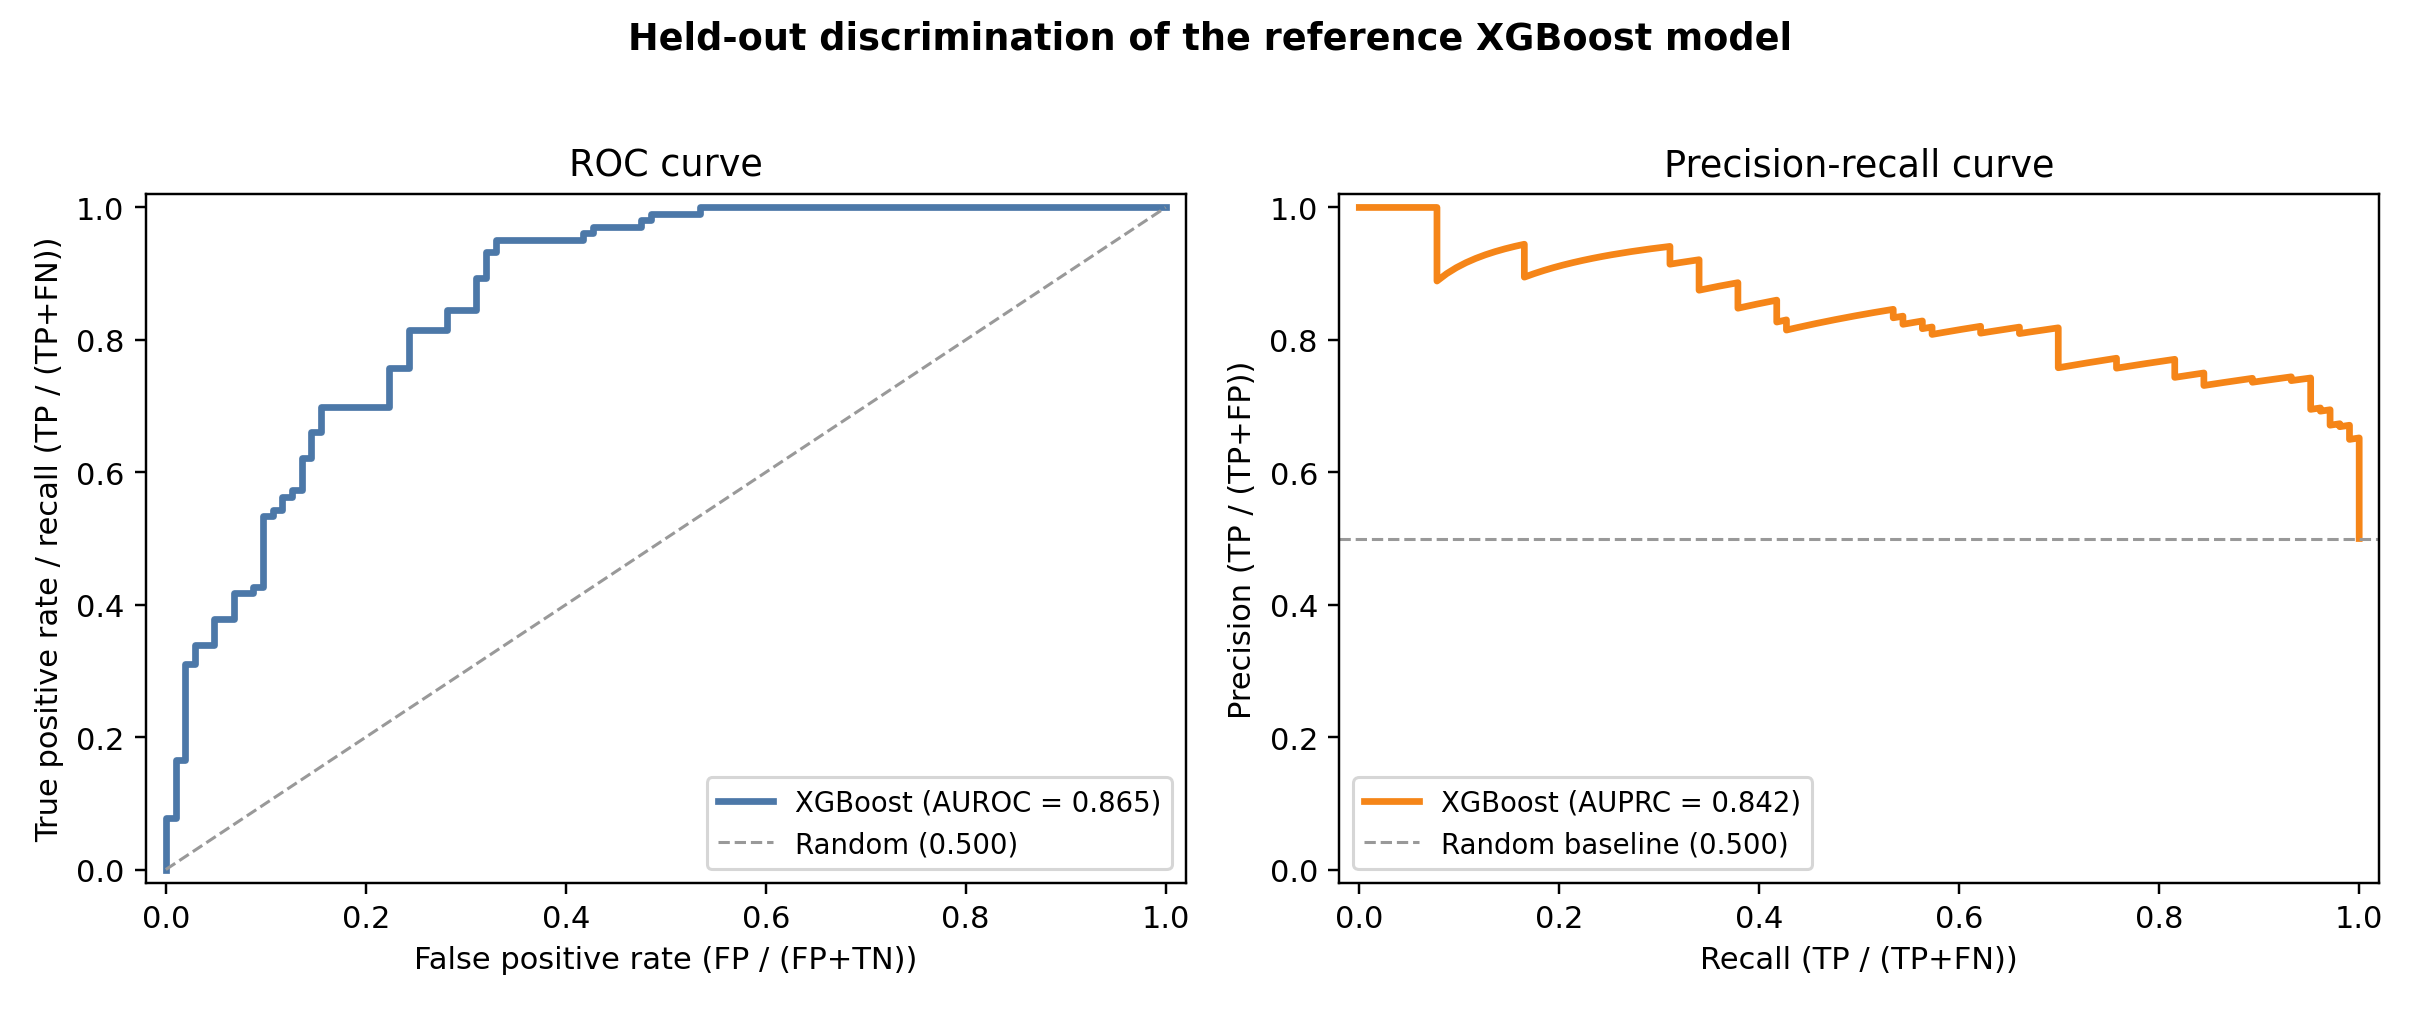
\includegraphics[width=\textwidth]{FigC_roc_pr.png}
\caption{\textbf{ROC and precision--recall curves for the reference XGBoost model} on the seed-42 outer-test split ($n=206$). Left: the ROC curve has AUROC $=0.865$. Right: the precision--recall curve has AUPRC $=0.842$, read against the random baseline of $0.500$ at the 1:1 ratio.}
\label{fig:roc_pr}
\end{figure}

Figure~\ref{fig:roc_pr} shows the two curves behind these summary numbers. The ROC curve reaches an AUROC of $0.865$, and the precision--recall curve gives an AUPRC of $0.842$ above the $0.500$ random baseline. At the default $0.5$ threshold the confusion matrix (Figure~\ref{fig:confusion}) records 87 true positives and 16 false negatives, with 71 true negatives and 32 false positives; precision is $0.731$, recall $0.845$, and F1 $0.784$.

\begin{figure}[H]
\centering
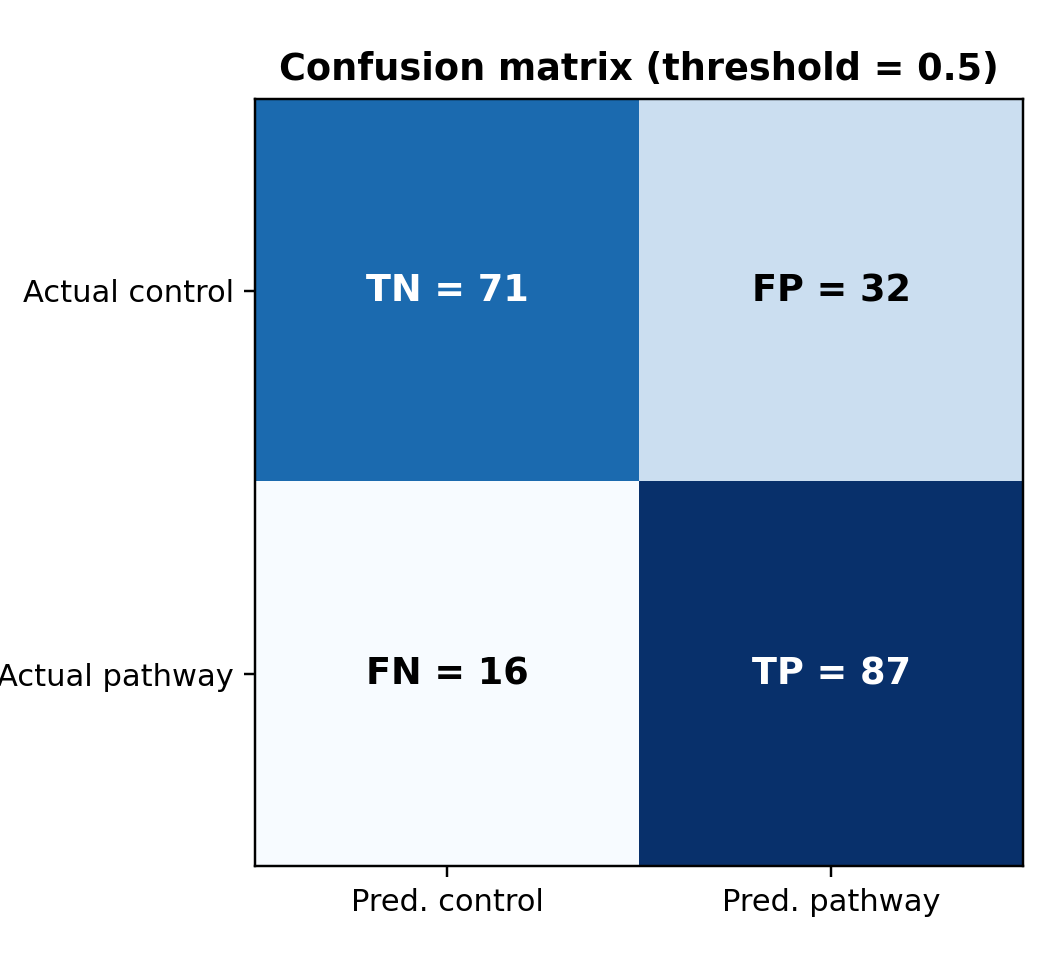
\includegraphics[width=0.56\textwidth]{FigF_confusion.png}
\caption{\textbf{Confusion matrix for the reference XGBoost model} at the default $0.5$ threshold on the 206 outer-test gene sets (103 curated pathway instances and 103 constructed controls).}
\label{fig:confusion}
\end{figure}

Breaking the held-out scores down by gene-set type (Figure~\ref{fig:score_by_type}) shows where the difficulty lies. Median scores are lowest for random and shuffled controls ($0.009$ and $0.010$) and highest for curated pathways ($0.794$); the two hard negatives fall in between, at $0.684$ for partial pathways and $0.510$ for cross-pathway mixtures. All 32 false positives come from these two groups: 19 partial and 13 cross-pathway controls. Against random and shuffled controls alone, AUROC is $0.996$ and $0.997$, respectively; it falls to $0.656$ for partial pathways and $0.809$ for cross-pathway mixtures.

\begin{figure}[H]
\centering

\includegraphics[width=0.9\textwidth]{FigG_score_by_type.png}
\caption{\textbf{Outer-test model score by gene-set type.} Box plots (with individual points) of the reference XGBoost score for the 206 test sets, split by the curated positives and four constructed negative types. Random and shuffled controls receive low scores, whereas partial pathways and cross-pathway mixtures lie closer to the $0.5$ threshold (dashed line).}
\label{fig:score_by_type}
\end{figure}

\section{GO feature-selection stability}
\label{sec:res_go_stability}

The nested CV runs also show how much the selected GO terms depend on the
training fold. For the 1:1 ratio, the mean pairwise Jaccard similarity between
the 15 selected-term sets was 0.123. Three terms were selected in all 15 folds,
and 15 terms appeared in at least half of the folds. XGBoost AUROC was more
stable than the term lists ($0.838 \pm 0.023$). The model therefore gives
reasonably stable predictions without producing a fixed biological GO
signature.

\section{SHAP feature attribution}
\label{sec:res_shap}

To understand what drives the predictions, we applied SHAP TreeExplainer \citep{lundberg2017unified} to the held-out test set. For each sample, SHAP values $\phi_i$ (log-odds units) quantify the contribution of feature $i$; global importance is the mean $|\phi_i|$ across all samples (Table~\ref{tab:shap}; Figure~\ref{fig:shap}).

The three most important features are mean Jaccard similarity, GO-profile entropy, and annotated gene count. The high importance of \texttt{jaccard\_mean} is consistent with the intended feature design and shows that the fitted model relies strongly on pairwise GO annotation overlap. Co-expression analyses arrive at gene relatedness from a different angle, grouping genes by correlated expression \citep{langfelder2008wgcna,liesecke2018ranking}; here the shared annotation is measured directly, as an explicit learnable feature rather than inferred from expression.

\begin{figure}[H]
\centering
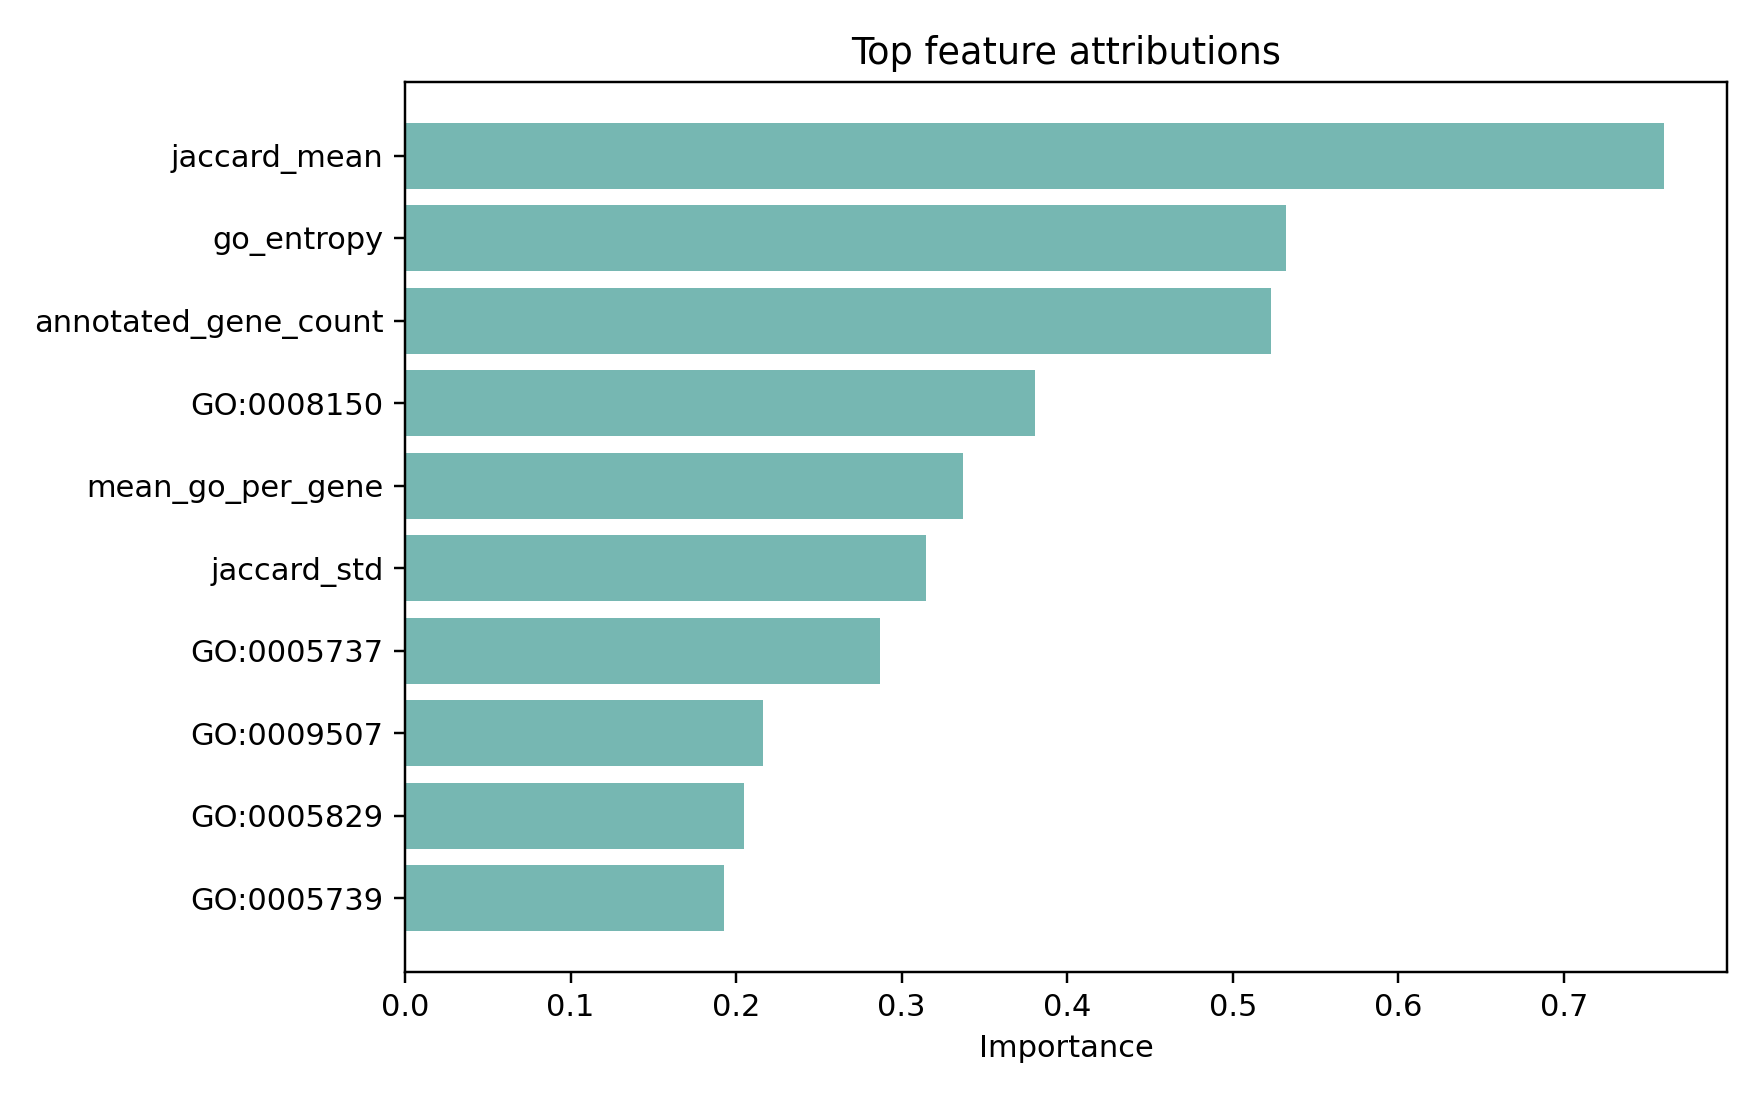
\includegraphics[width=0.92\textwidth]{Fig3_shap.png}
\caption{\textbf{SHAP feature attribution for the XGBoost model.}
\texttt{jaccard\_mean}, \texttt{go\_entropy}, and \texttt{annotated\_gene\_count} are the top three predictors on the held-out split.}
\label{fig:shap}
\end{figure}


\begin{table}[H]
\centering
\caption{\textbf{Top 10 features by attribution on the held-out test split.}
Importance is mean absolute SHAP value for tree-based attribution.}
\label{tab:shap}
\setlength{\tabcolsep}{5pt}
\renewcommand{\arraystretch}{1.2}
\begin{tabular}{cllc}
\toprule
\textbf{Rank} & \textbf{Feature} & \textbf{Type} & \textbf{Importance} \\
\midrule
1 & \texttt{jaccard\_mean} & Jaccard & 0.760 \\
2 & \texttt{go\_entropy} & size/statistic & 0.532 \\
3 & \texttt{annotated\_gene\_count} & size/statistic & 0.523 \\
4 & \texttt{GO:0008150} & GO term & 0.381 \\
5 & \texttt{mean\_go\_per\_gene} & size/statistic & 0.337 \\
6 & \texttt{jaccard\_std} & Jaccard & 0.315 \\
7 & \texttt{GO:0005737} & GO term & 0.287 \\
8 & \texttt{GO:0009507} & GO term & 0.216 \\
9 & \texttt{GO:0005829} & GO term & 0.205 \\
10 & \texttt{GO:0005739} & GO term & 0.193 \\
\bottomrule
\end{tabular}
\end{table}


\section{Feature-group ablation}
\label{sec:res_ablation}

To measure the contribution of each feature group, we trained XGBoost on subsets of the 69 features using the same held-out split (Table~\ref{tab:s3_ablation}). Using any one group alone costs 0.055--0.133 AUROC, whereas dropping a single group costs only 0.026--0.045. The full 69-feature model has the highest AUROC, with the surviving groups partly covering for whichever one is left out.

\begin{table}[H]
\centering
\caption{\textbf{Feature-group ablation using XGBoost.}
$\Delta$ is the difference from the full model's test AUROC.}
\label{tab:s3_ablation}
\renewcommand{\arraystretch}{1.18}
\setlength{\tabcolsep}{7pt}
\begin{tabular}{lrrrr}
\toprule
\textbf{Configuration} & $d$ & \textbf{Test AUROC} & \textbf{AUPRC} & $\boldsymbol{\Delta}$ AUROC \\
\midrule
Full model & 69 & 0.865 & 0.842 & 0.000 \\
GO only & 60 & 0.810 & 0.763 & $-$0.055 \\
Jaccard only & 4 & 0.732 & 0.710 & $-$0.133 \\
Size/entropy only & 5 & 0.778 & 0.712 & $-$0.087 \\
$-$GO frequency & 9 & 0.820 & 0.782 & $-$0.045 \\
$-$Jaccard & 65 & 0.838 & 0.815 & $-$0.026 \\
$-$Size/entropy & 64 & 0.837 & 0.794 & $-$0.028 \\
\bottomrule
\end{tabular}
\end{table}


\chapter{Discussion}
\label{sec:discussion}

The results show that GO-derived features can separate curated \textit{Arabidopsis} pathway instances from constructed controls with moderate-to-good accuracy (test AUROC 0.865, AUPRC 0.842). Some controls still contain real biological signals, making this benchmark harder than using purely random data. The nested-CV and ablation results show that the performance is not explained by one split or one feature group alone.

\section{Understanding the performance level}
\label{sec:disc_performance}

The held-out AUROC of 0.865 should be read in light of the benchmark design. If the negative class contained only random gene sets, performance would be higher but biologically less meaningful. The present benchmark mixes four negative types---random, shuffled, partial, and cross-pathway---each testing a different failure mode. Partial pathways retain genuine functional coherence because they are subsets of real pathways. Their median score of 0.684 and negative-type AUROC of 0.656 show that they are the main boundary case. The overall result reflects the difficulty of distinguishing complete curated pathways from partially coherent alternatives.

Raw AUPRC cannot be compared across class ratios without considering its random baseline \citep{saito2015precision}. The ratio comparison was therefore run only within the outer training set, with fold-specific GO selection. The 1:1 ratio had the highest mean normalised AUPRC (0.561) and F1 (0.786). Mean AUROC ranged from 0.825 to 0.845, and the largest difference from 1:1 was 0.65 pooled SD. Taken together, the two metrics pointed to 1:1 for the final outer-test analysis. Normalisation adjusts AUPRC relative to its random baseline, but it does not make precision--recall performance invariant to prevalence.

\section{Feature-selection variation}
\label{sec:disc_feature_variation}

The selected GO terms changed across CV folds. For the 1:1 analysis, the mean pairwise Jaccard similarity between term sets was 0.123, and only three terms appeared in every fold. The corresponding AUROC SD was 0.023. This suggests that several GO subsets can support similar predictive performance. The selected terms should therefore be read as features of the fitted model, not as a universal biological signature.

\section{Interpreting SHAP features and broad GO terms}
\label{sec:disc_shap_interpretation}

\texttt{jaccard\_mean} dominates the SHAP ranking (0.760), showing that the fitted model leans heavily on pairwise GO overlap. Behind it, \texttt{go\_entropy} (0.532) tracks whether the selected-GO profile is concentrated on a few terms or spread across many, and \texttt{annotated\_gene\_count} (0.523) matters because small sets provide limited pairwise evidence while very large sets often correspond to broad KEGG overview maps. These values are mean absolute SHAP contributions in model-output units and should be compared within this fitted model rather than interpreted as probabilities.

Among the GO term features, GO:0008150 (biological process) ranks fourth overall, GO:0005737 (cytoplasm) ranks seventh, and GO:0009507 (chloroplast) ranks eighth. GO:0008150 is broad, and its SHAP contribution may partly reflect annotation depth rather than a specific process. Specific GO terms and Jaccard features should therefore be considered alongside broad terms and size-related features.

\section{Relationship to enrichment analysis}
\label{sec:disc_practical_workflow}

PathwayML-Ath is meant to sit alongside ORA and GSEA. Enrichment methods test whether a gene list overlaps a known pathway catalogue; PathwayML-Ath asks whether the list has internal coherence resembling curated pathways. The two questions are different and can be combined in a practical workflow: (a)~run ORA/GSEA to check for known pathway enrichment; (b)~score the gene set with PathwayML-Ath; (c)~inspect SHAP features to understand what drives the score; (d)~compare the set against known pathways by maximum Jaccard similarity; (e)~prioritise only modules where the score, enrichment profile, and biological context are consistent.

This workflow reduces the risk of over-interpreting model scores. A gene set that is strongly enriched for a known pathway and also receives a high PathwayML-Ath score can be interpreted as a coherent known-pathway-related module. A set with a high PathwayML-Ath score but no enrichment hit may represent an uncurated coherent module, but that interpretation requires literature support and experimental validation before it can be treated as a biological finding.

\section{Implications for plant functional genomics}
\label{sec:disc_plant_implications}

Plant transcriptomic experiments routinely produce gene modules that are not yet represented in curated databases. A GO-based coherence score can help sort such modules: high-scoring modules with interpretable SHAP profiles deserve deeper analysis, while low-scoring modules may reflect mixed regulation, sparse annotation, or non-pathway processes. This is especially useful for abiotic stress studies, where responses often involve hormone signalling, detoxification, transport, and transcriptional regulation co-induced without forming a single curated pathway. Combined-stress experiments in particular typically produce modules that mix several response programmes, making coherence scoring a practical first filter.

\section{Limitations}
\label{sec:disc_limitations}

Four main limitations apply.
(i)~\textbf{GO annotation incompleteness.}
GO coverage varies across \textit{Arabidopsis} genes, reducing sensitivity for poorly characterised gene sets. Foundation models such as ESM-2 and related protein-language models \citep{lin2023evolutionary} could supply sequence-derived representations for unannotated genes.
(ii)~\textbf{No graph topology.}
The model treats each gene set as a bag of features and does not exploit protein--protein interaction or regulatory network structure. Graph neural networks \citep{muzio2021biological} could capture topological signals once dense \textit{Arabidopsis} interactomes become available.
(iii)~\textbf{Unimodal features.}
The representation is GO-centric. Multi-omics integration---transcriptomic, proteomic, metabolomic---has improved module discovery in animal systems \citep{hasin2017multiomics} and would be a natural extension for plant studies.
(iv)~\textbf{Database dependence.}
The model uses the fixed database releases and files listed in Table~\ref{tab:s5_data}. These resources change over time, so the model should be retrained when a new release is adopted. A calibrated confidence estimate could also help users judge individual scores.

Besides these four points, there are other limitations to the feature representation.

The feature representation deliberately prioritises interpretability over completeness. It does not model reaction direction, enzyme order, metabolite connectivity, protein interactions, transcription-factor binding, expression dynamics, or subcellular timing. A gene set may therefore be mechanistically coherent yet score low if its coherence is not reflected in GO annotations. Conversely, a gene set may score high because its members share broad GO terms (e.g.\ ``cytosol'' or ``biological\_process'') without forming a mechanistically coherent pathway. As discussed in Section~\ref{sec:disc_shap_interpretation}, SHAP inspection helps distinguish these cases, but the model score alone cannot guarantee biological specificity.

The outer held-out benchmark is free of supervised feature-selection leakage: the variance filter and mutual-information ranking see only the primary training records, and controls are generated separately on the train and test sides. Repeated CV also reruns the label-dependent selection steps inside each fold. However, the low overlap between fold-specific GO lists shows that the feature identities are sensitive to the training sample. Performance was more stable than the selected term lists, so biological interpretation should focus on recurrent GO terms or broader functional themes rather than one fixed GO signature.

Finally, pathway definitions are not fixed. Database updates, pathway-size filters, and duplicate handling can all change the training set. This study uses a KEGG REST snapshot archived on 25 May 2026, when Release 118.1 was current, and the AraCyc 18.0.0 flat file from PMN Release 16, dated 21 October 2025. The filtered sources contain 538 records, grouped into 512 unique gene-set instances. Exact grouping prevents identical gene sets from appearing on both sides of the split, but near-duplicate pathways remain. Some large KEGG overview maps also represent broader biology than a narrow metabolic module.

\section{Future directions}
\label{sec:disc_future_work}

Five extensions would strengthen the framework.

\textbf{Pathway universe versioning.} The training set depends on specific database snapshots. Archiving these snapshots and comparing results across alternative pathway-universe definitions (e.g.\ excluding broad KEGG overview maps, including Reactome plant pathways, or using updated AraCyc releases) would quantify how sensitive the model is to the composition of the positive class. A systematic comparison of full-source, filtered-source, and overview-map-excluded settings would also clarify whether very large KEGG maps should be treated as standard positives or handled separately.

\textbf{Richer feature representations.} The current GO-based features are interpretable but incomplete. Co-expression edge densities from resources such as ATTED-II \citep{obayashi2018atted}, protein interaction densities from STRING or BioGRID, reaction graph connectivity, and protein language model embeddings \citep{lin2023evolutionary} could capture aspects of pathway biology that GO frequency and Jaccard statistics miss. Deep learning on plant genomic sequences may also provide complementary representations for genes with sparse GO annotation. A rigorous comparison would require using the same train/test splits and negative controls, so that performance differences can be attributed to the feature representation rather than to experimental design differences.

\textbf{External validation.} The current outer split is independent, but both sides come from the same KEGG and AraCyc snapshots. A future release or another curated plant pathway resource would provide a stronger external test. Such a test should preserve the same negative definitions and rerun feature selection using only its training data.

\textbf{Uncertainty estimation.} The present model outputs a score but provides no formal confidence interval. Extra calibration or a Bayesian treatment could turn the raw score into a probability, helping users separate high-confidence prioritisation calls from borderline ones. This would be especially valuable in an applied setting where experimental follow-up resources are limited.

\textbf{Cross-species transfer.} The model is trained exclusively on \textit{Arabidopsis} pathways and GO annotations. Extending it to crop species (rice, maize, wheat) would require re-mapping pathway databases, adjusting for differences in annotation depth, and validating against species-specific pathway collections for those crops. Transfer learning or domain adaptation strategies could help bridge annotation gaps between well-annotated model organisms and less-characterised crops.

Future work should keep the benchmark and interpretation rules fixed when new features are compared. Otherwise, a change in performance cannot be assigned to the new representation alone.


\chapter{Conclusion}
\label{sec:conclusion}

PathwayML-Ath is a supervised framework that scores gene sets for pathway-like coherence in \textit{Arabidopsis thaliana}. The 538 KEGG and AraCyc source records were grouped into 512 unique gene-set modelling instances and encoded as 69-dimensional GO annotation vectors. The XGBoost reference model achieves nested-CV AUROC $0.838 \pm 0.023$ and outer-test AUROC $0.865$ (AUPRC $0.842$). SHAP analysis identifies pairwise GO Jaccard similarity, annotation entropy, and annotated gene count as the main predictors. The score can be combined with ORA or GSEA in downstream applications; on its own it is not evidence of a new pathway. All scripts, generated tables, figures, and provenance metadata are provided in the project archive.


\appendix

\chapter{Terminology Guide}
\label{app:terminology}

\begin{description}[style=nextline,leftmargin=1.5em]
\item[Pathway] A curated set of genes, proteins, and metabolites that execute a defined biological process. Here, 538 KEGG/AraCyc records are grouped into 512 unique gene-set instances for modelling.
\item[Gene module] Any set of genes grouped by analysis (differential expression, co-expression, clustering, etc.). A module may match a known pathway, overlap several, or represent an uncurated process.
\item[Pathway-like coherence] The degree to which a gene set resembles curated pathways in GO-derived feature space. This is a model-defined score, not mechanistic proof.
\item[Candidate gene set] An experimental gene set submitted for scoring. A high score indicates resemblance to curated pathways; it does not confirm a novel pathway without independent evidence.
\item[Negative gene set] Constructed controls (random, shuffled, partial, mixed) used for training. These are not verified non-pathways.
\item[Score interpretation] Scores are comparative. Values near 1 indicate strong resemblance to curated pathways; values near 0 indicate weak resemblance. Intermediate values may reflect partial coherence, mixed membership, or sparse annotation.
\end{description}

\chapter{Reproducibility Checklist}
\label{app:repro_checklist}

\begin{enumerate}[leftmargin=*]
  \item Archive or checksum KEGG, AraCyc, and TAIR GO source files; report data snapshots.
  \item Record the pathway inventory (identifier, source, name, gene count, and exact gene-set group).
  \item Record the GO mapping (annotated genes, unique terms, deduplicated pairs).
  \item Save selected GO terms and filtering counts for each analysis run.
  \item Record negative type, source pathway, size, and split assignment.
  \item Record all model hyperparameters in the manifest.
  \item Report random seed values for splits, negative sampling, and model fitting.
  \item Use values from generated tables, not manually copied values.
  \item Match each LaTeX figure to a code-generated figure or label it as schematic.
\end{enumerate}

The project archive contains generated tables, figures, software versions, and provenance metadata corresponding to the source-file analysis (538 source records, 512 modelling groups, 69 features, XGBoost outer-test AUROC 0.865).

\chapter{Metrics}
\label{app:metrics}

AUROC measures the probability that a random positive scores higher than a random negative; it is useful for overall ranking but can appear stable under class imbalance. AUPRC focuses on positive-class precision and recall and is more informative when false positives are costly \citep{saito2015precision}. F1 summarises precision and recall at a fixed threshold. In this thesis, AUROC compares discrimination across models, AUPRC evaluates positive-class ranking quality, and nested CV measures variation across training folds.


\chapter*{Acknowledgements}
The author thanks the maintainers of KEGG, PlantCyc/AraCyc, TAIR, and the Gene Ontology resource for maintaining publicly accessible biological databases. The author also thanks project supervisors and reviewers for feedback on the computational workflow and thesis.

\chapter*{Data Availability Statement}
KEGG pathway names and pathway--gene links were obtained from the REST endpoints
\url{https://rest.kegg.jp/list/pathway/ath} and
\url{https://rest.kegg.jp/link/ath/pathway}. AraCyc data came from PMN/PlantCyc
(\url{https://plantcyc.org/data-downloads/}). GO annotations came from the TAIR
Public Data Releases (\url{https://arabidopsis.org/download/}). The accompanying
project archive contains the source files, checksums, analysis scripts, generated
tables and figures, software-version records, and provenance metadata.

% ===================  REFERENCES  ===================
\begin{singlespace}
\bibliographystyle{unsrtnat}
\bibliography{references}
\end{singlespace}

\end{document}
